\documentclass{beamer}
\usepackage{ctex}
\usepackage{hyperref}
\usepackage[T1]{fontenc}

% other packages
\usepackage{latexsym,amsmath,xcolor,multicol,booktabs,calligra}
\usepackage{graphicx,pstricks,listings,stackengine}
\usepackage[backend=bibtex,sorting=none]{biblatex}

% settings
\addbibresource{ref.bib}
\setbeamerfont{footnote}{size=\tiny}
\ctexset{
    today=old,
    figurename=Figure,
    tablename=Table
}


\author{Sicun Li}
\title{Imaging Pipeline Reconfiguration for UAV-Based Correlation Filter Tracking}
\subtitle{面向无人机相关滤波跟踪的成像流水线重构}
\institute{School of Microelectronics}
\date{\today}
\usepackage{dlut}

% defs
\def\cmd#1{\texttt{\color{red}\footnotesize $\backslash$#1}}
\def\env#1{\texttt{\color{blue}\footnotesize #1}}
\definecolor{deepblue}{rgb}{0,0,0.5}
\definecolor{deepred}{rgb}{0.6,0,0}
\definecolor{deepgreen}{rgb}{0,0.5,0}
\definecolor{halfgray}{gray}{0.55}

\lstset{
    basicstyle=\ttfamily\small,
    keywordstyle=\bfseries\color{deepblue},
    emphstyle=\ttfamily\color{deepred},    % Custom highlighting style
    stringstyle=\color{deepgreen},
    numbers=left,
    numberstyle=\small\color{halfgray},
    rulesepcolor=\color{red!20!green!20!blue!20},
    frame=shadowbox,
}


\begin{document}

% titlepage
\begin{frame}
    \titlepage
\end{frame}

\begin{frame}
    \frametitle{Outline}
    \tableofcontents[sectionstyle=show,subsectionstyle=show/shaded/hide,subsubsectionstyle=show/shaded/hide]
\end{frame}

\section{Background \& Motivation}

\subsection{Imaging Pipeline}

\begin{frame}
    \begin{figure}[htpb]
        \begin{center}
            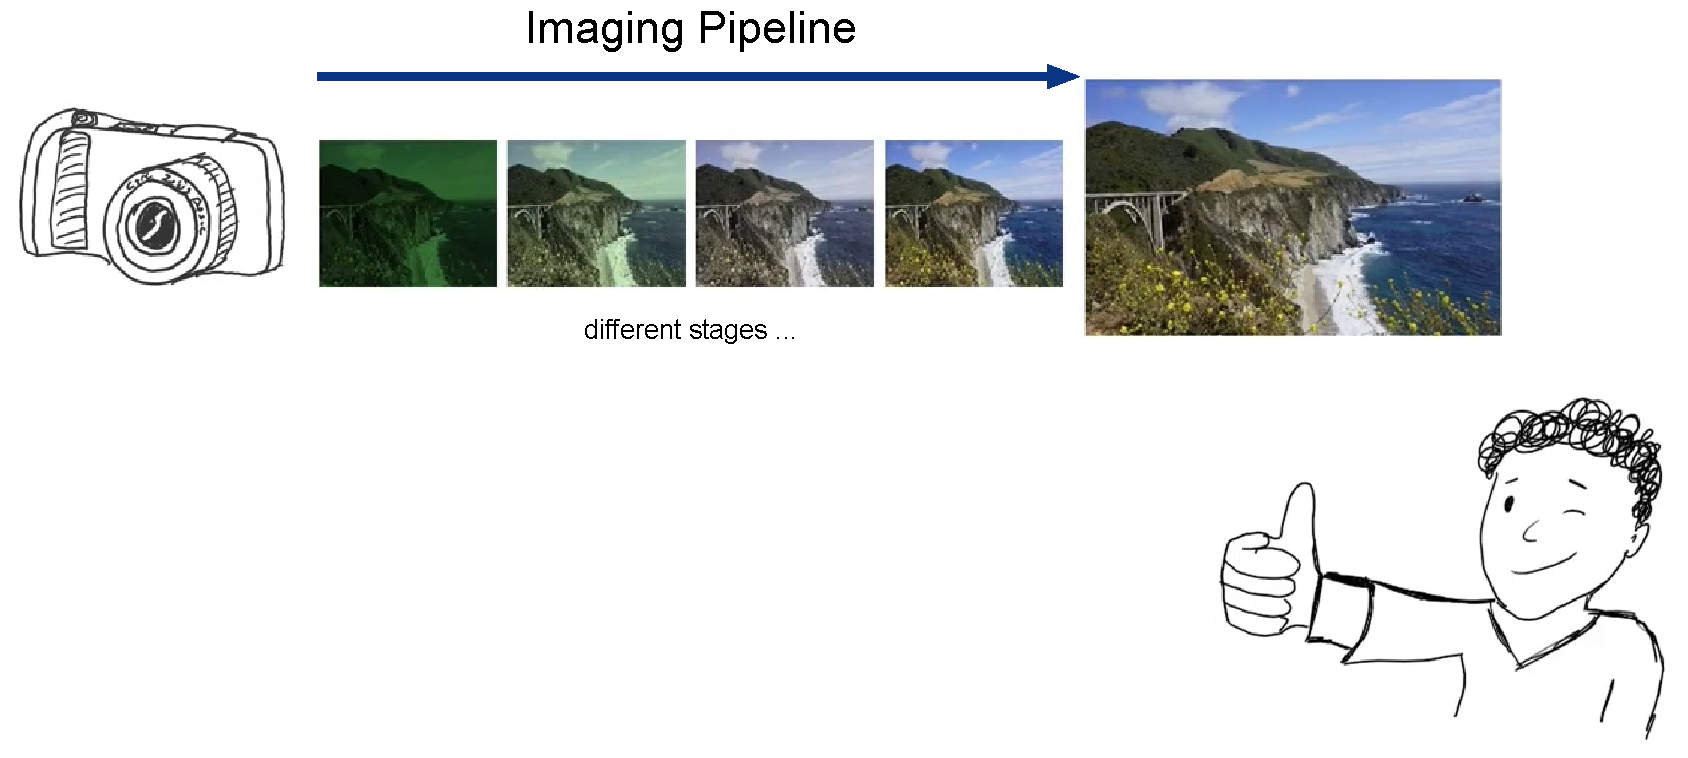
\includegraphics[width=1.0\linewidth]{fig/isp0.pdf}
        \end{center}
    \end{figure}
\end{frame}

\begin{frame}
    \begin{figure}[htpb]
        \begin{center}
            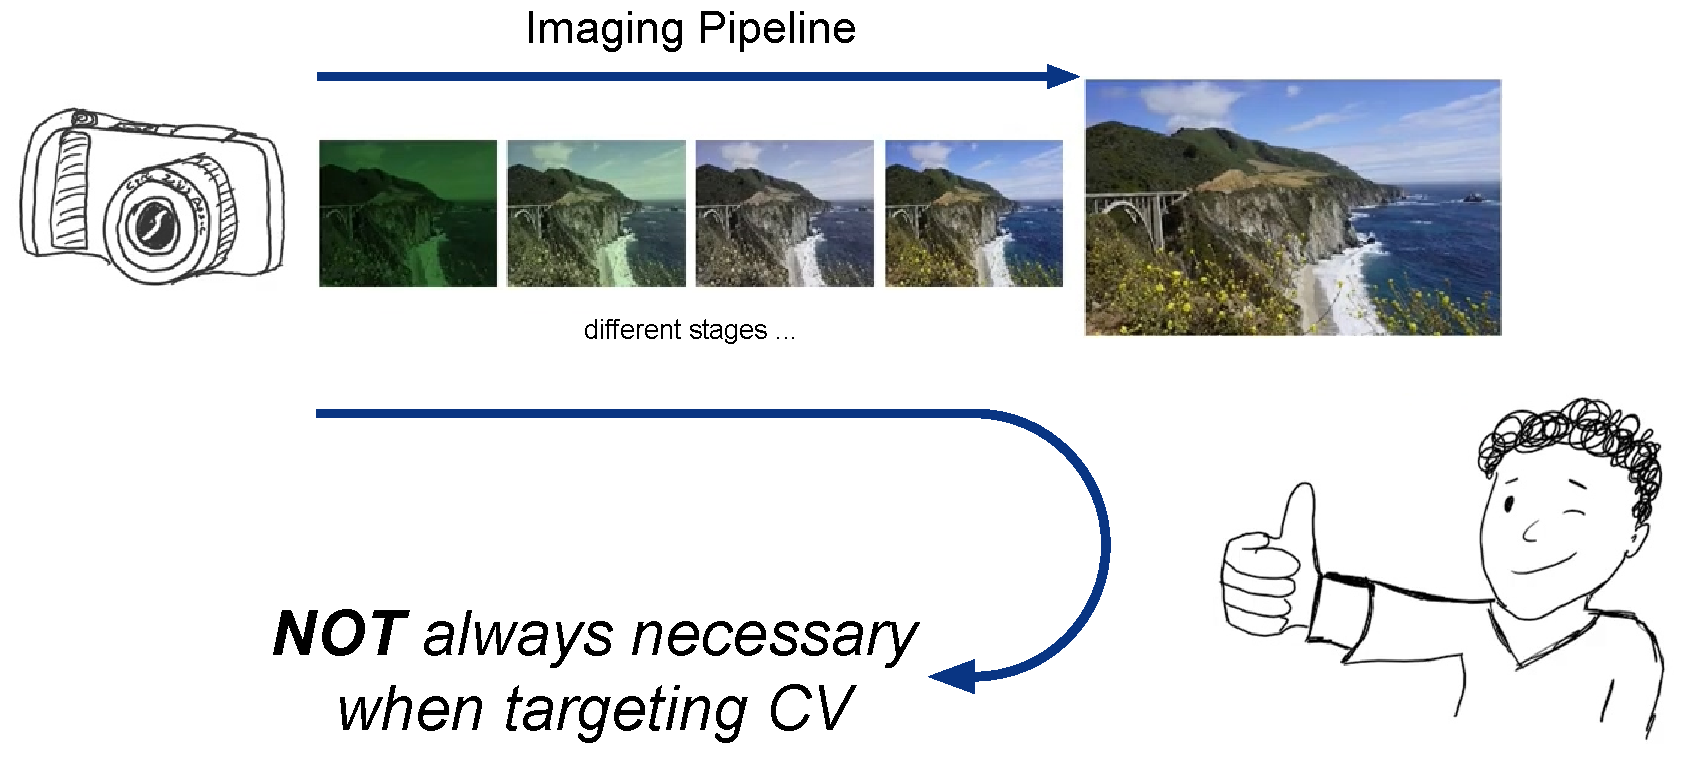
\includegraphics[width=1.0\linewidth]{fig/isp1.pdf}
        \end{center}
    \end{figure}
\end{frame}

\subsection{UAV-Based Correlation Filter Tracking}

\begin{frame}
    Object Tracking:
    \begin{figure}[htpb]
        \begin{center}
            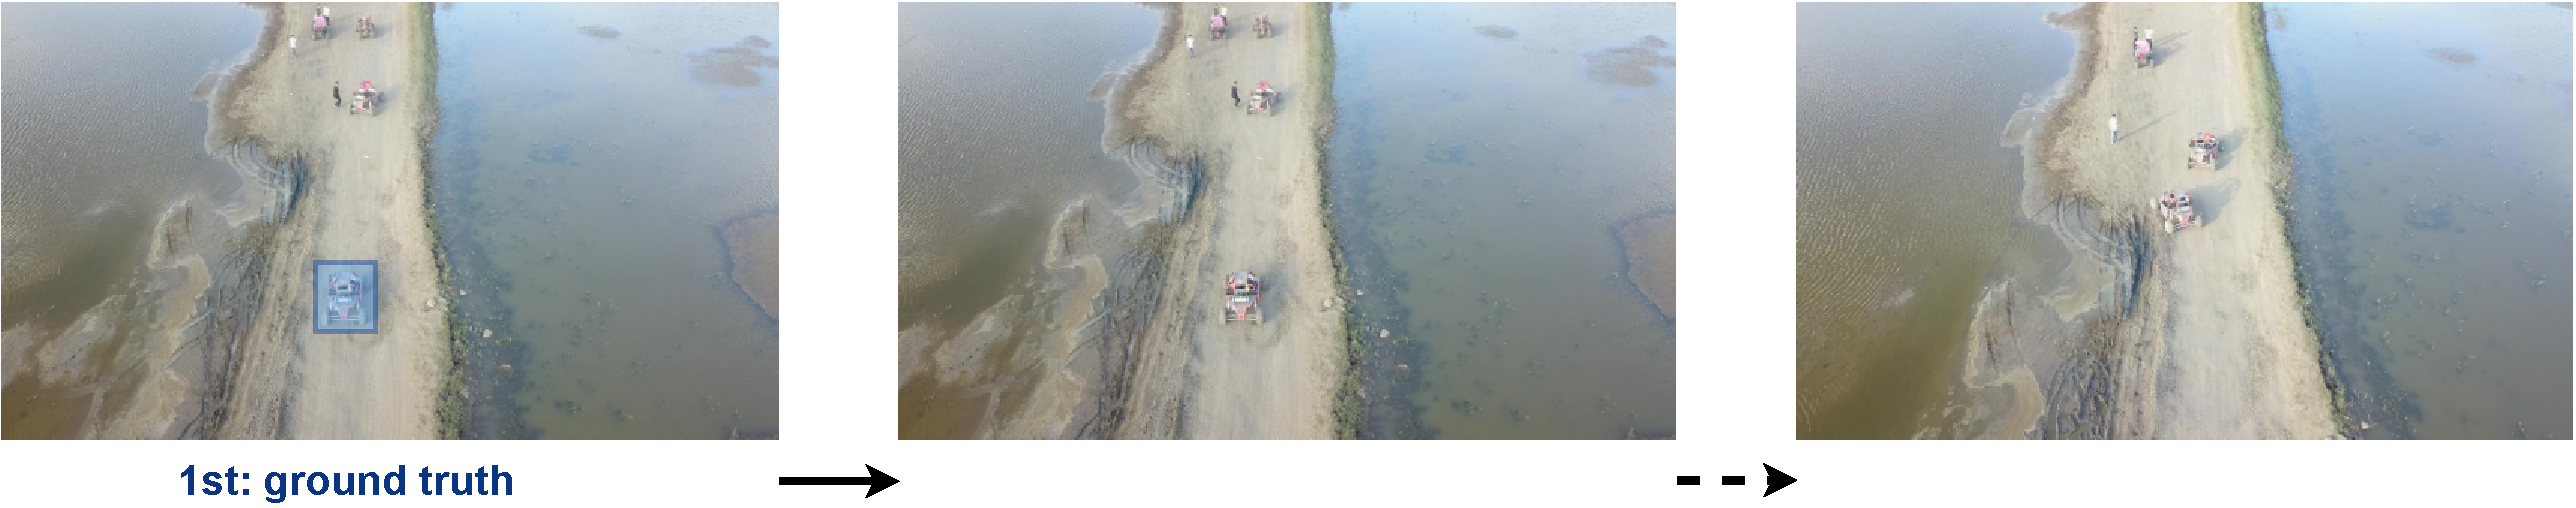
\includegraphics[width=1.0\linewidth]{fig/obt0.pdf}
        \end{center}
    \end{figure}
\end{frame}

\begin{frame}
    Object Tracking:
    \begin{figure}[htpb]
        \begin{center}
            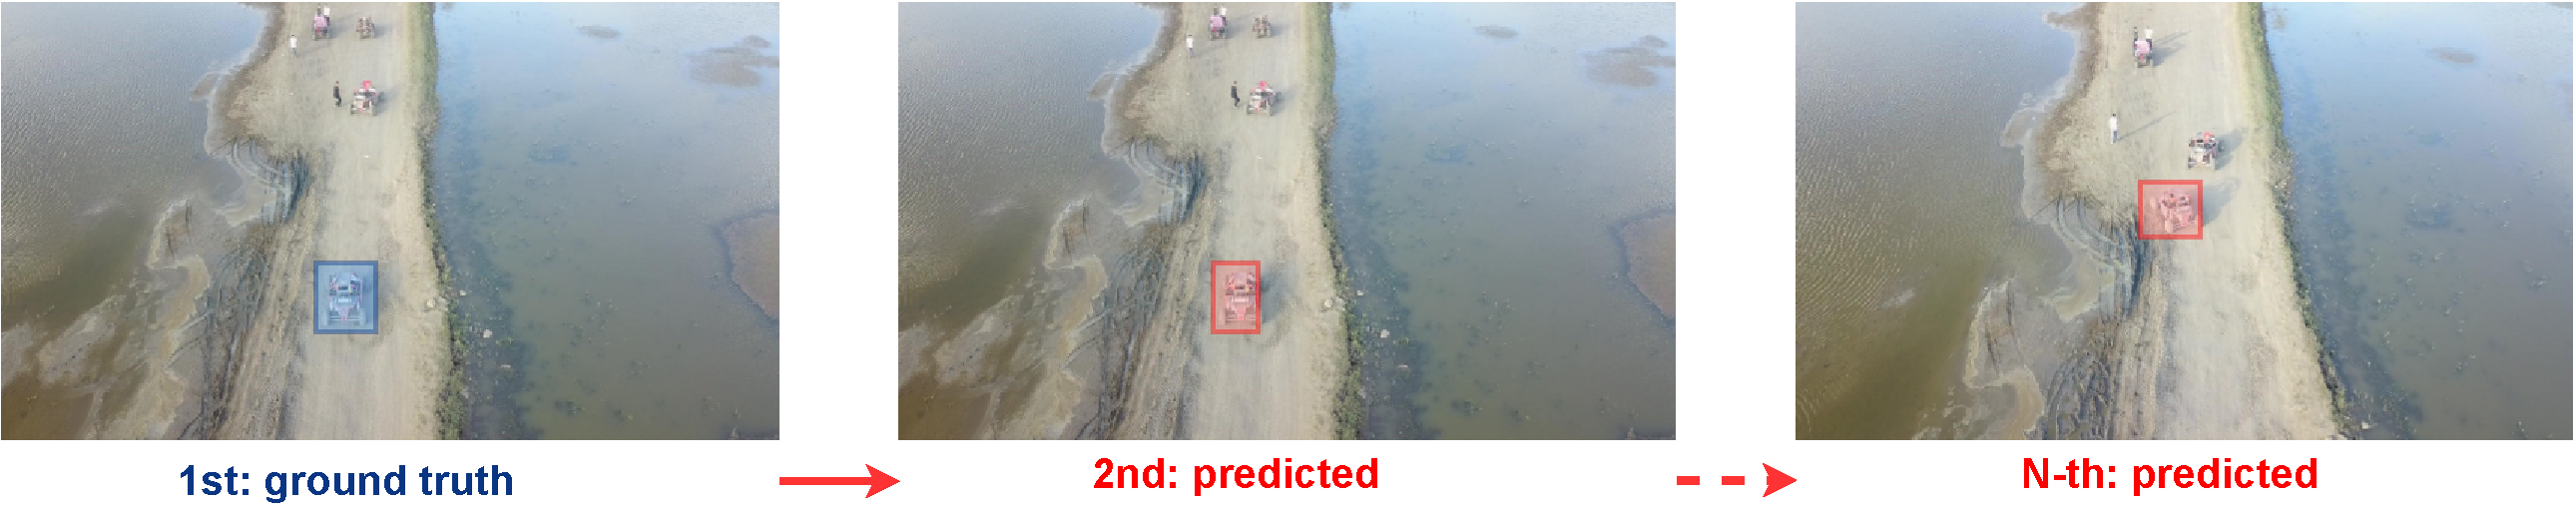
\includegraphics[width=1.0\linewidth]{fig/obt1.pdf}
        \end{center}
    \end{figure}
\end{frame}

\begin{frame}
    \begin{itemize}[<+-| alert@+>]
        \item Generative methods: to learn how to describe the state of the target.
        \item Discriminative methods: to train a classifier that can distinguish the tracking object from the background.
    \end{itemize}
\end{frame}

\begin{frame}

    General tracking structure of DCF-based methods onboard the UAV platform\footfullcite{fu2021correlation}:

    \begin{figure}[htpb]
        \begin{center}
            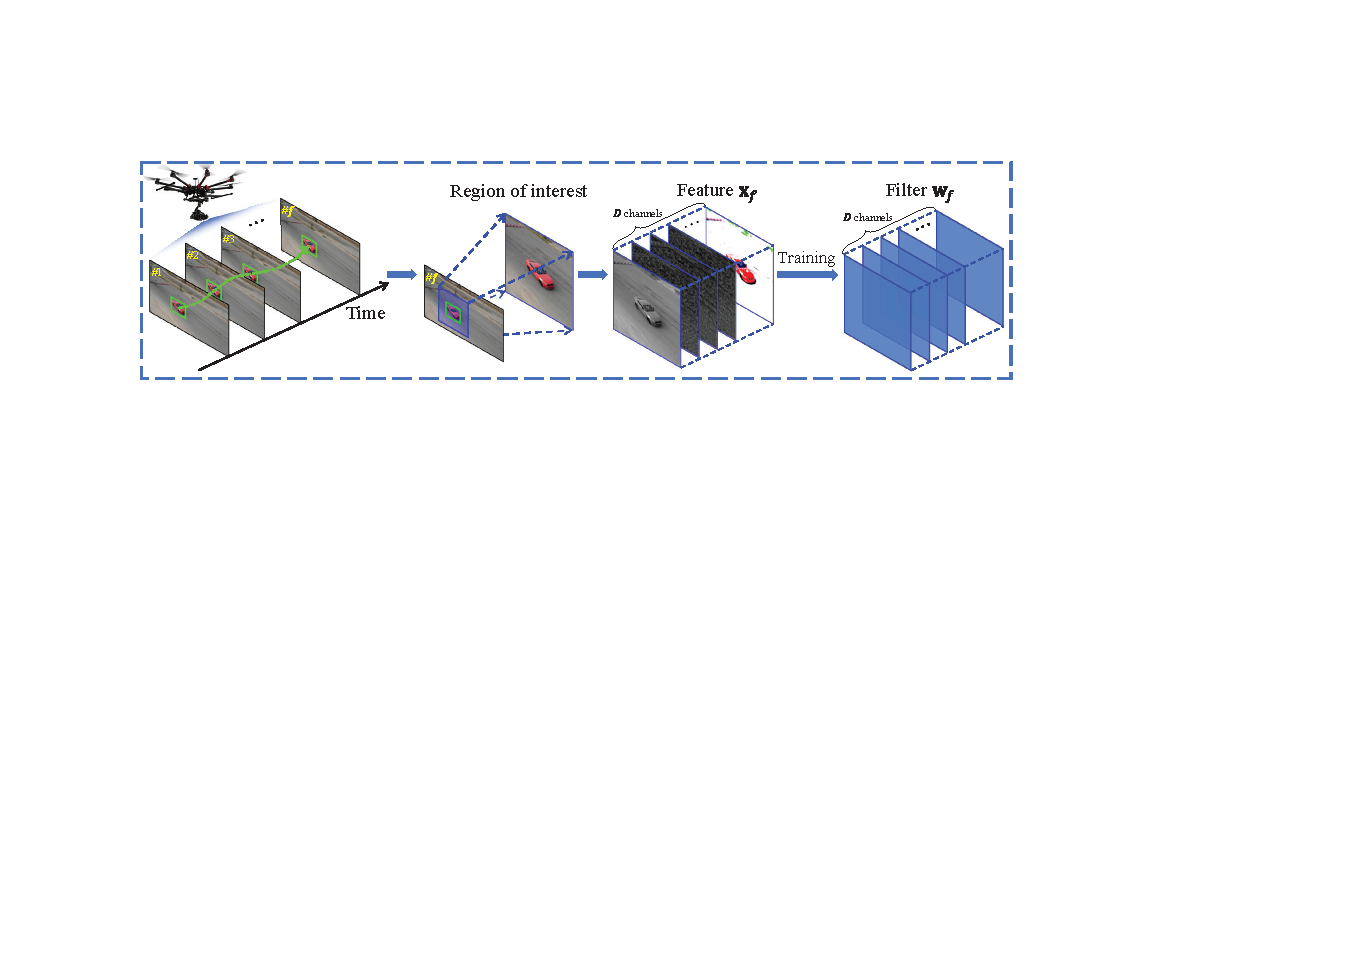
\includegraphics[width=0.7\linewidth, trim={100pt 100 100 90}]{fig/tracking_1.pdf}
        \end{center}
    \end{figure}

    which can be divided into the \textcolor{red}{training stage}, model update, and detection stage.

\end{frame}

\begin{frame}

    \addtocounter{footnote}{-1}
    \addtocounter{framenumber}{-1}
    General tracking structure of DCF-based methods onboard the UAV platform\footfullcite{fu2021correlation}:

    \begin{figure}[htpb]
        \begin{center}
            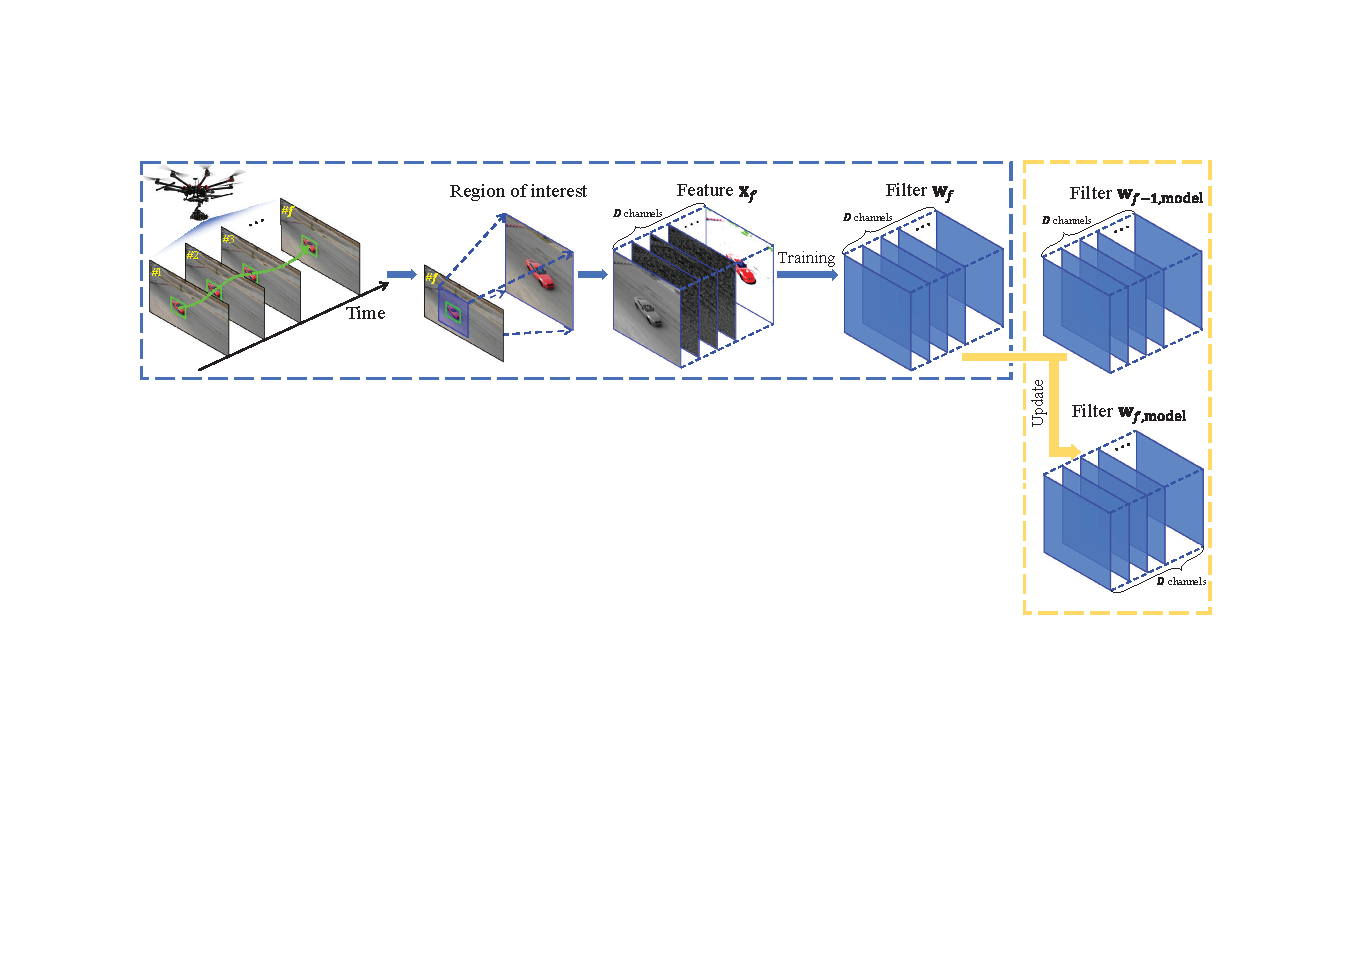
\includegraphics[width=0.7\linewidth, trim={100pt 100 100 90}]{fig/tracking_2.pdf}
        \end{center}
    \end{figure}

    which can be divided into the training stage, \textcolor{red}{model update}, and detection stage.

\end{frame}

\begin{frame}

    \addtocounter{footnote}{-1}
    \addtocounter{framenumber}{-1}
    General tracking structure of DCF-based methods onboard the UAV platform\footfullcite{fu2021correlation}:

    \begin{figure}[htpb]
        \begin{center}
            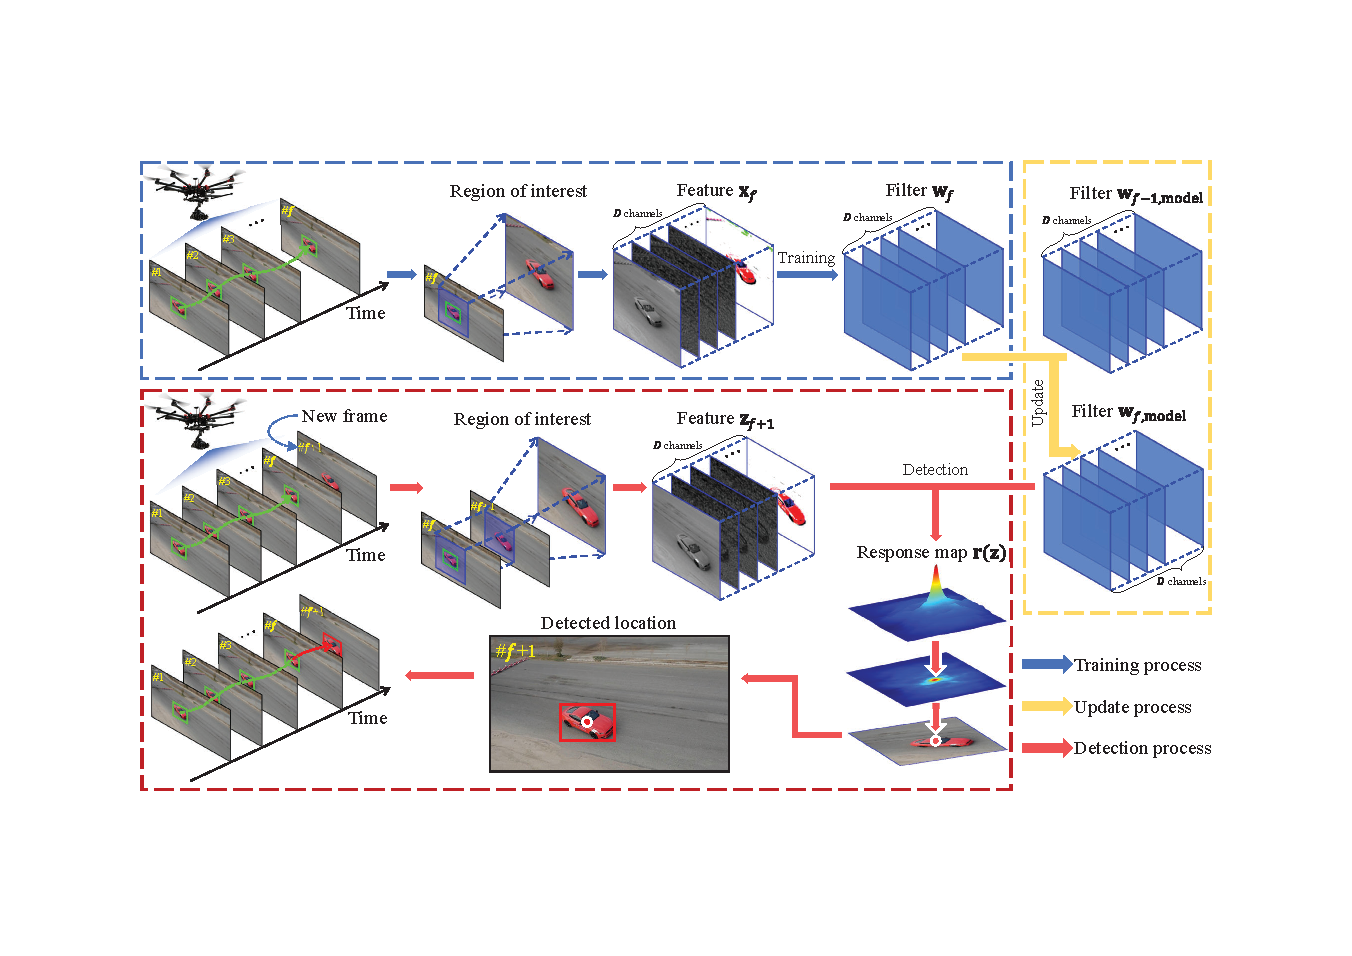
\includegraphics[width=0.7\linewidth, trim={100pt 100 100 90}]{fig/tracking_3.pdf}
        \end{center}
    \end{figure}

    which can be divided into the training stage, model update, and \textcolor{red}{detection stage}.

\end{frame}

\begin{frame}
    Why DCF is suitable for UAVs:
    \begin{itemize}
        \item \textcolor{red}{Adaptability:} DCF is an online learning method, the tracking model is usually updated once every frame.
        \item \textcolor{red}{Robustness:} The DCF-based method belongs to the discriminative method. It not only learns the object information but also the background information. 
        \item \textcolor{red}{Efficiency:} Most of the operations involved in DCF are element-wise products in the frequency domain.
    \end{itemize}
\end{frame}

\subsection{The Entire System}

\begin{frame}
    \begin{figure}[htpb]
        \begin{center}
            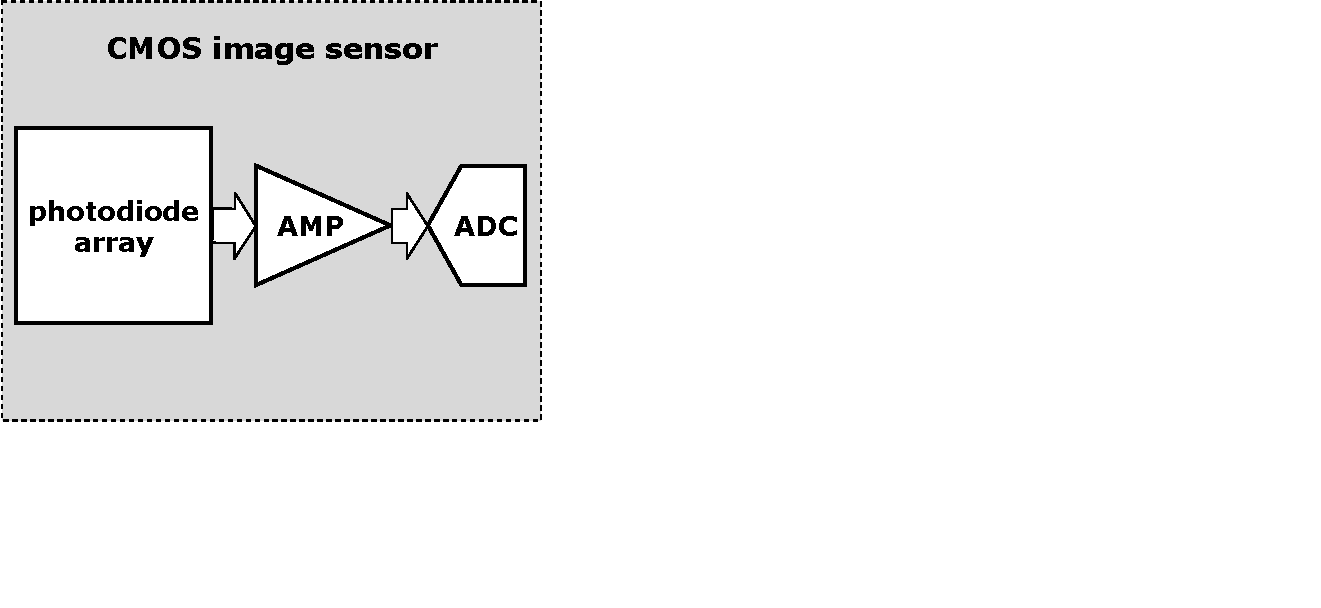
\includegraphics[width=1.0\linewidth]{fig/block0.pdf}
        \end{center}
    \end{figure}
\end{frame}

\begin{frame}
    \begin{figure}[htpb]
        \begin{center}
            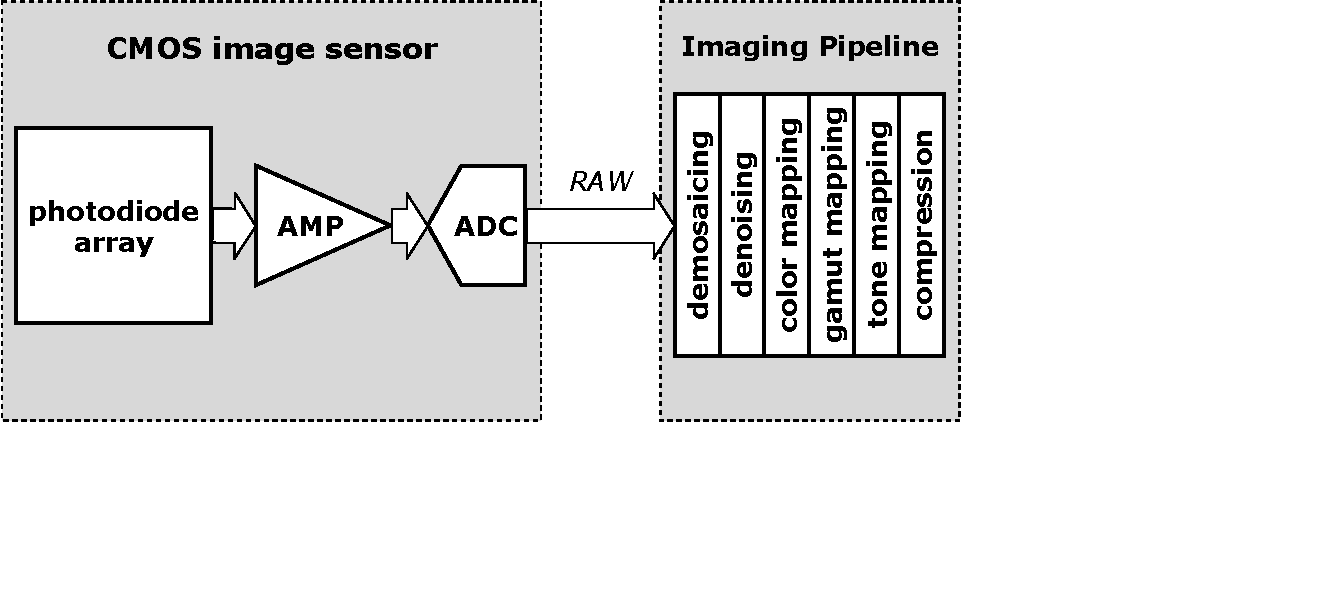
\includegraphics[width=1.0\linewidth]{fig/block1.pdf}
        \end{center}
    \end{figure}
\end{frame}

\begin{frame}
    \begin{figure}[htpb]
        \begin{center}
            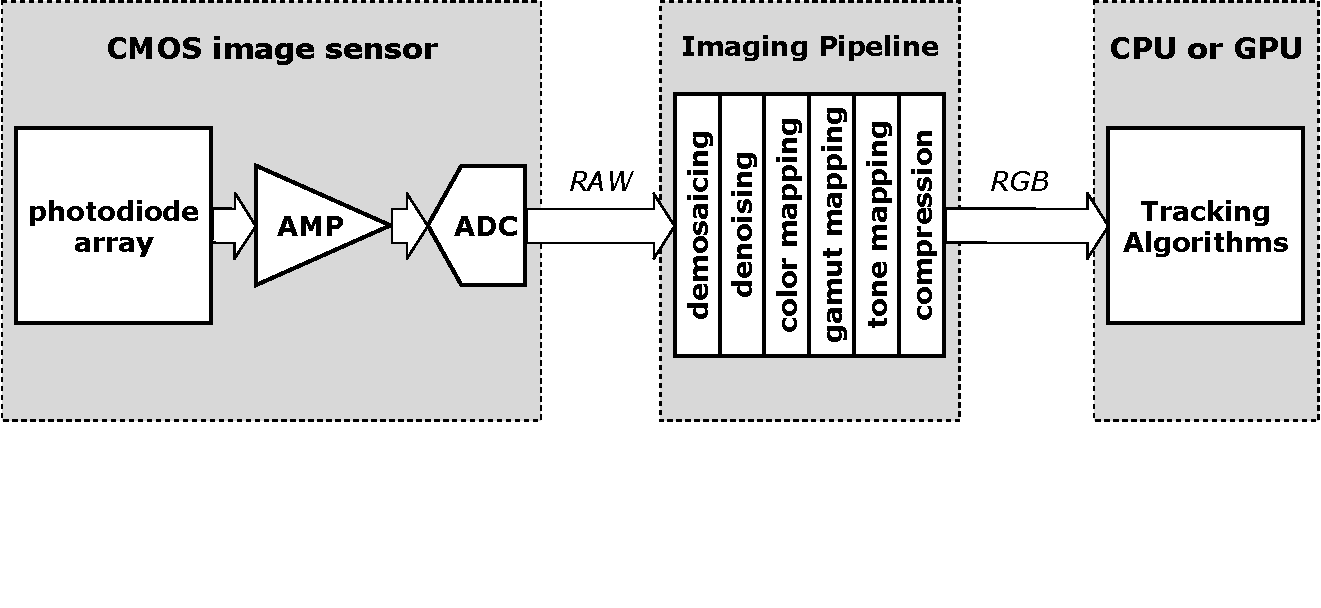
\includegraphics[width=1.0\linewidth]{fig/block2.pdf}
        \end{center}
    \end{figure}
\end{frame}

\begin{frame}
    \begin{figure}[htpb]
        \begin{center}
            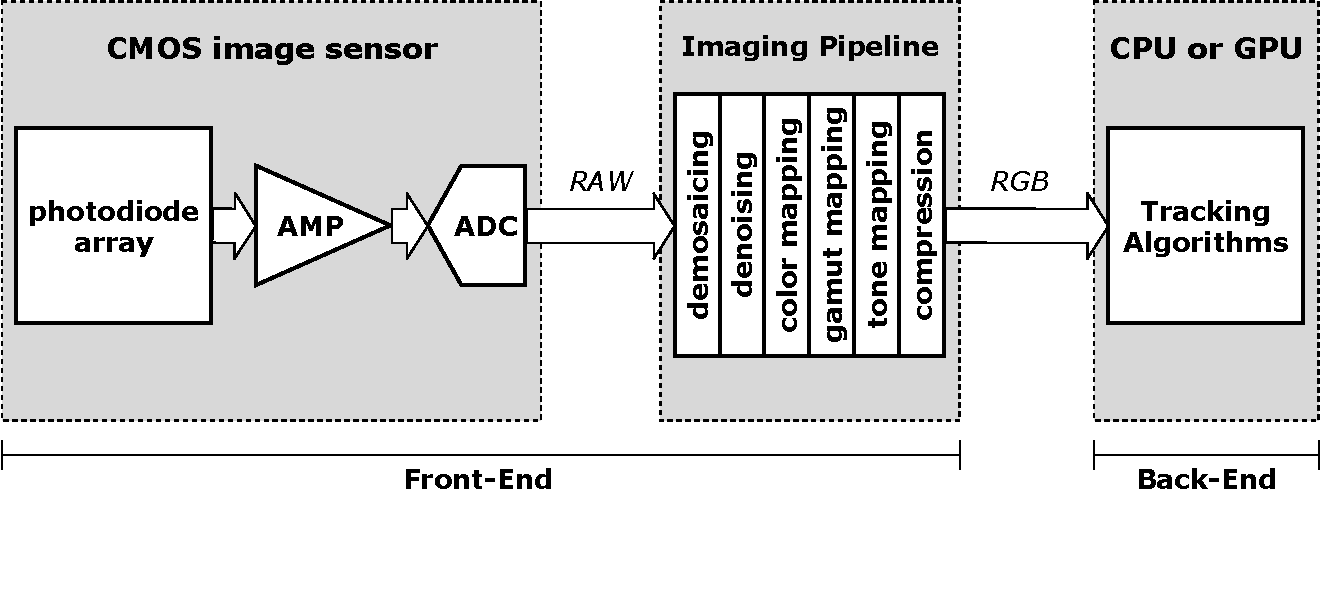
\includegraphics[width=1.0\linewidth]{fig/block3.pdf}
        \end{center}
    \end{figure}
\end{frame}

\begin{frame}
    However, such system is bottlenecked by
    \begin{itemize}
        \item long end-to-end latency
        \item and excessive power consumption of the Front-End.
    \end{itemize}
    \textcolor{red}{It's necessary to optimize the Front-End of the entire system to reduce latency and power consumption\footfullcite{gan2020low}.}
\end{frame}

\begin{frame}
    \begin{figure}[htpb]
        \begin{center}
            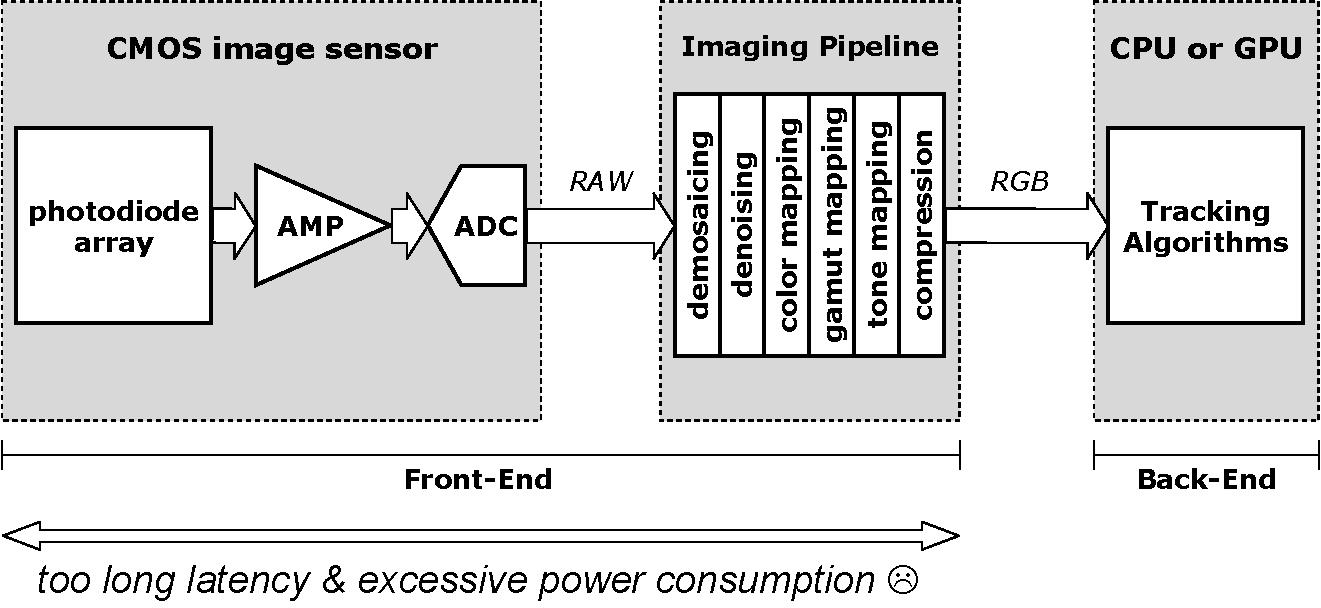
\includegraphics[width=1.0\linewidth]{fig/block4.pdf}
        \end{center}
    \end{figure}
\end{frame}

\subsection{Related Work}

% \begin{frame}

%     Zhenhong Liu et al. show that only \textcolor{red}{gamma correction} and \textcolor{red}{demosicking} stages are critical for a \textcolor{red}{face detection} algorithm they adopt\footfullcite{liu2015ultra}.

% \end{frame}

% \begin{frame}
    
%     Mark Buckler et al. show that \textcolor{red}{for both CNN-based and classical vision algorithms}, only two ISP stages, \textcolor{red}{demosaicing} and \textcolor{red}{gamma compression}, are critical for task performance.
    
%     \vspace{0.3in}
    
%     They then use a subsampling circuitry and 5-bit logarithmic ADC to approximate the effects of these two ISP stages and can even disable the ISP altogether\footfullcite{buckler2017reconfiguring}.

% \end{frame}

% \begin{frame}
    
%     Researchers of Intel have proposed VisionISP\footfullcite{wu2019visionisp}, primarily for deep convolutional neural networks, which significantly reduces the bit-number and resolution of images using only noise reduction, tone mapping, and feature perception modules.
    
%     \vspace{0.3in}
    
%     Ekdeep Singh Lubana et al. propose an ISP architecture that includes only gamma transform and pixel binning from the perspective of matching intensity distributions, thus reducing the impact on the recognition accuracy of off-the-shelf DNNs\footfullcite{lubana2019minimalistic}.

% \end{frame}

\begin{frame}
    \begin{itemize}[<+-| alert@+>]
        \item A series of work\footfullcite{liu2015ultra}\footfullcite{buckler2017reconfiguring}\footfullcite{wu2019visionisp}\footfullcite{lubana2019minimalistic} validate the possibility of reducing the latency and power consumption of the Front-End of the system by simplifying the ISP architecture without affecting the accuracy of the CV algorithms significantly.
        \item However, their work only evaluated on a limited range of CV tasks, and never considered object tracking algorithms.
        \item This work will continue their ideas and further investigate the sensitivity of the performance of the DCF-based trackers to the different stages of the imaging pipeline in the UAV scenario.
    \end{itemize}
\end{frame}

\section{Main Contents}

\subsection{Datasets \& Trackers}

% VisDrone2019-SOT
\begin{frame}
    \begin{figure}[htpb]
        \begin{center}
            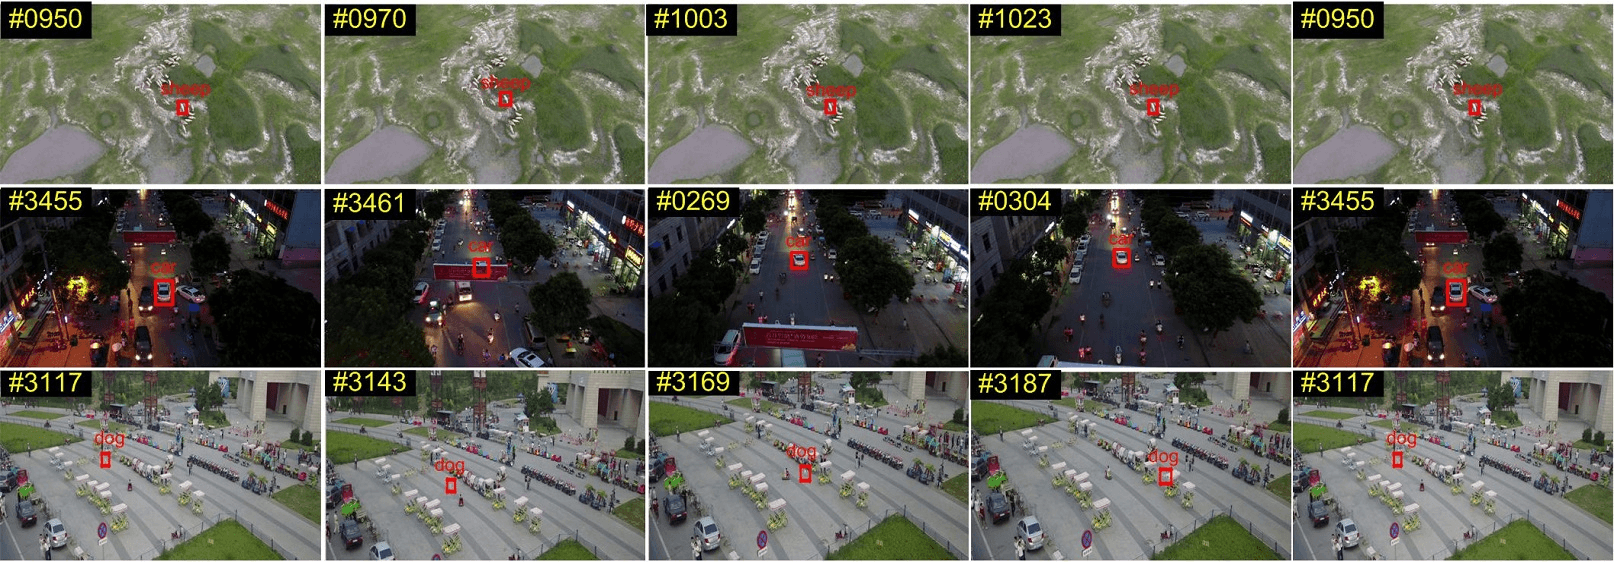
\includegraphics[width=1.0\linewidth]{fig/VisDrone.png}
            \caption{VisDrone2019-SOT Datasets\footfullcite{Du_2019_ICCV}}
        \end{center}
    \end{figure}
\end{frame}

% Tracker list
\begin{frame}
    \begin{table}[htpb]
        \centering
        \caption{Selected Trackers}
        \label{tab:number}
        \begin{tabular}{ccc}\toprule
            Name      & Venue     & Features                \\\midrule
            CN        & CVPR2014  & Grayscale + CN          \\
            KCF       & TPAMI2015 & fHOG                    \\
            Staple    & CVPR2016  & fHOG + Color historgram \\
            ECO-HC    & CVPR2017  & fHOG + CN               \\
            AutoTrack & CVPR2020  & fHOG + CN + Grayscale   \\\bottomrule
        \end{tabular}
    \end{table}
\end{frame}

\subsection{Imaging Pipeline Simulation Tool}

\begin{frame}

    Using the imaging pipeline simulation tool of Buckler et al.\footfullcite{buckler2017reconfiguring}
    
    \begin{figure}[htpb]
        \begin{center}
            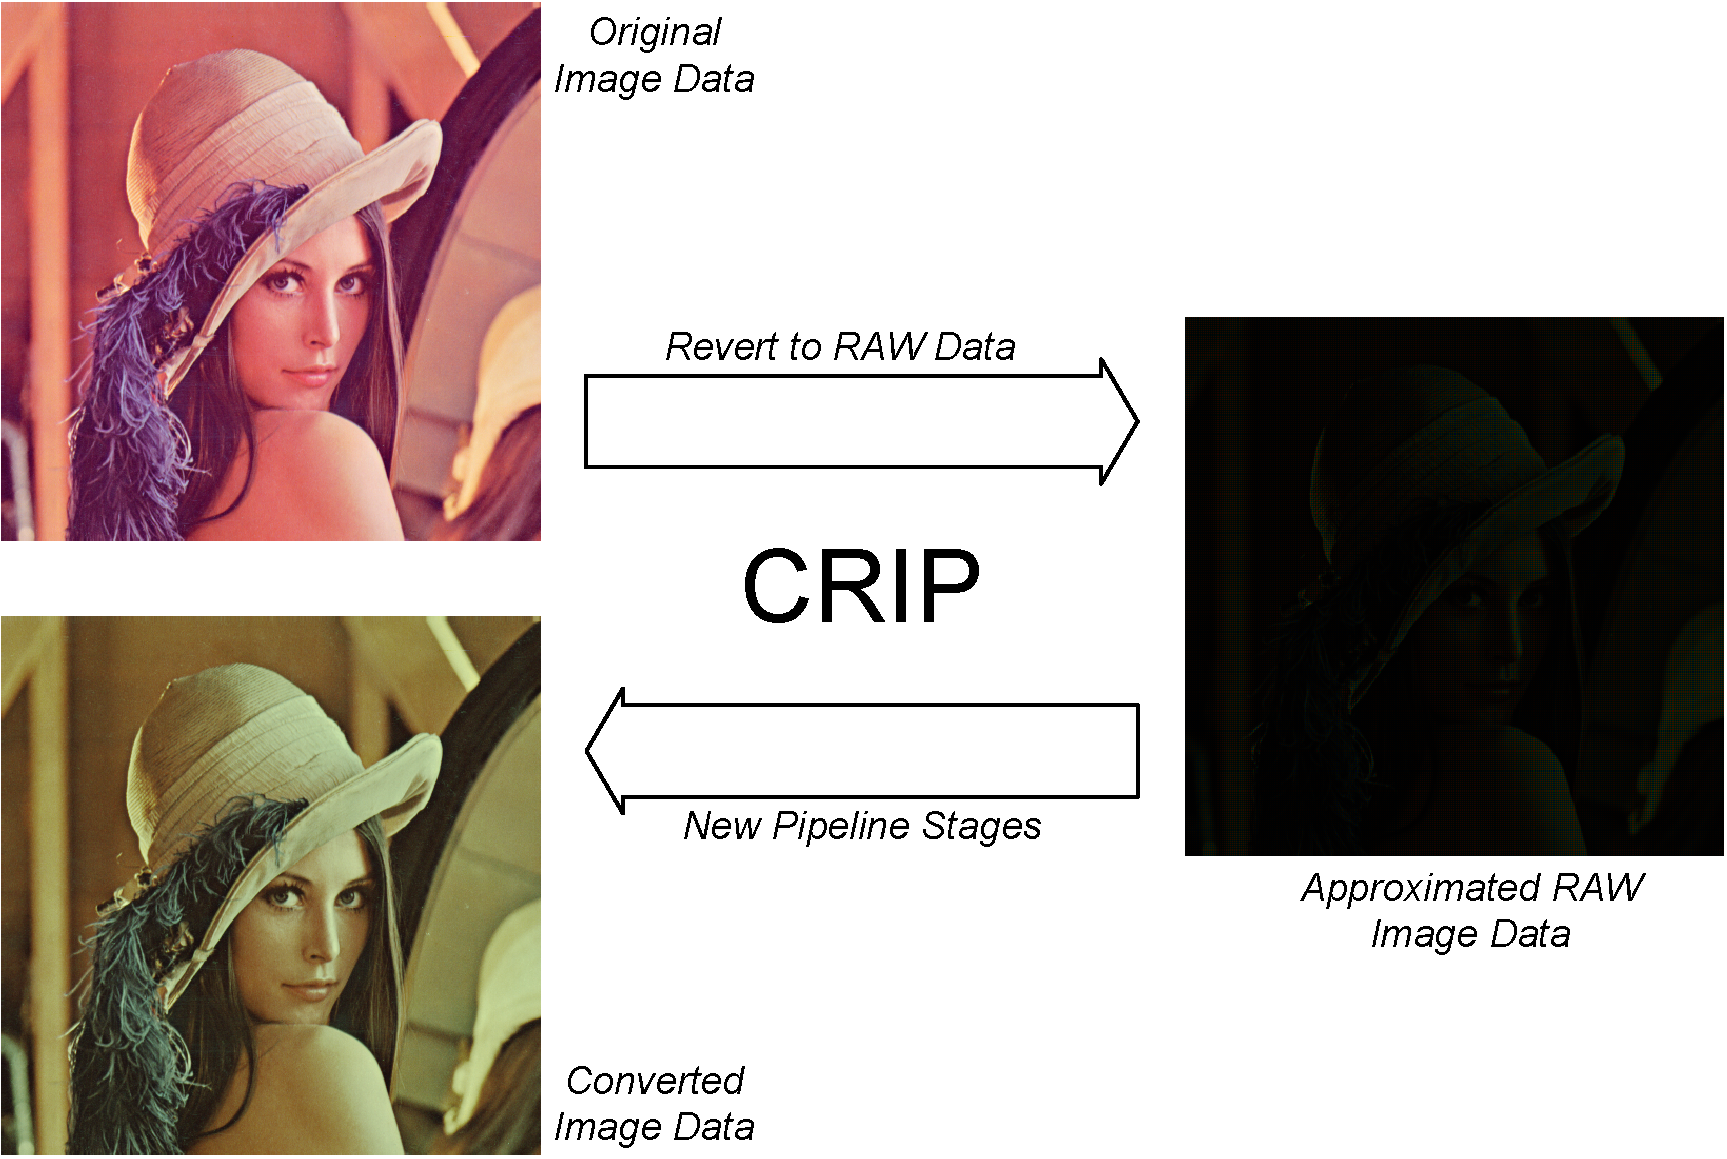
\includegraphics[width=0.65\linewidth]{fig/crip.pdf}
            \caption{Configurable \& Reversible Imaging Pipeline}
        \end{center}
    \end{figure}
\end{frame}

\subsection{Experimental Setup}

\begin{frame}
    \begin{figure}[htpb]
        \begin{center}
            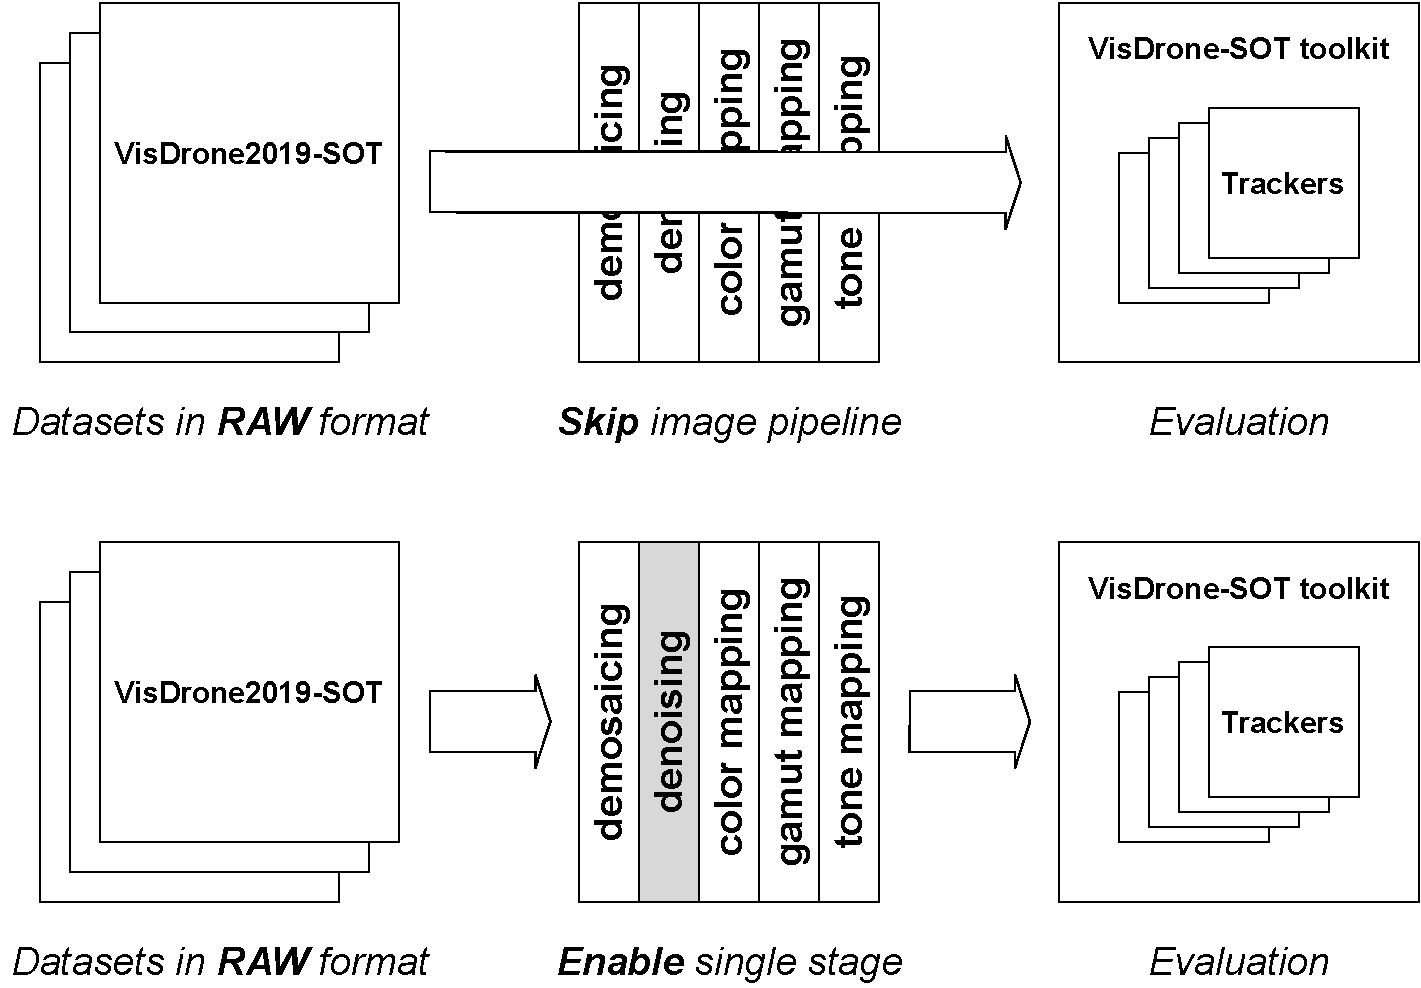
\includegraphics[width=0.8\linewidth]{fig/eva.pdf}
            \caption{all off vs. enable single stage}
        \end{center}
    \end{figure}
\end{frame}

\begin{frame}
    \begin{figure}[htpb]
        \begin{center}
            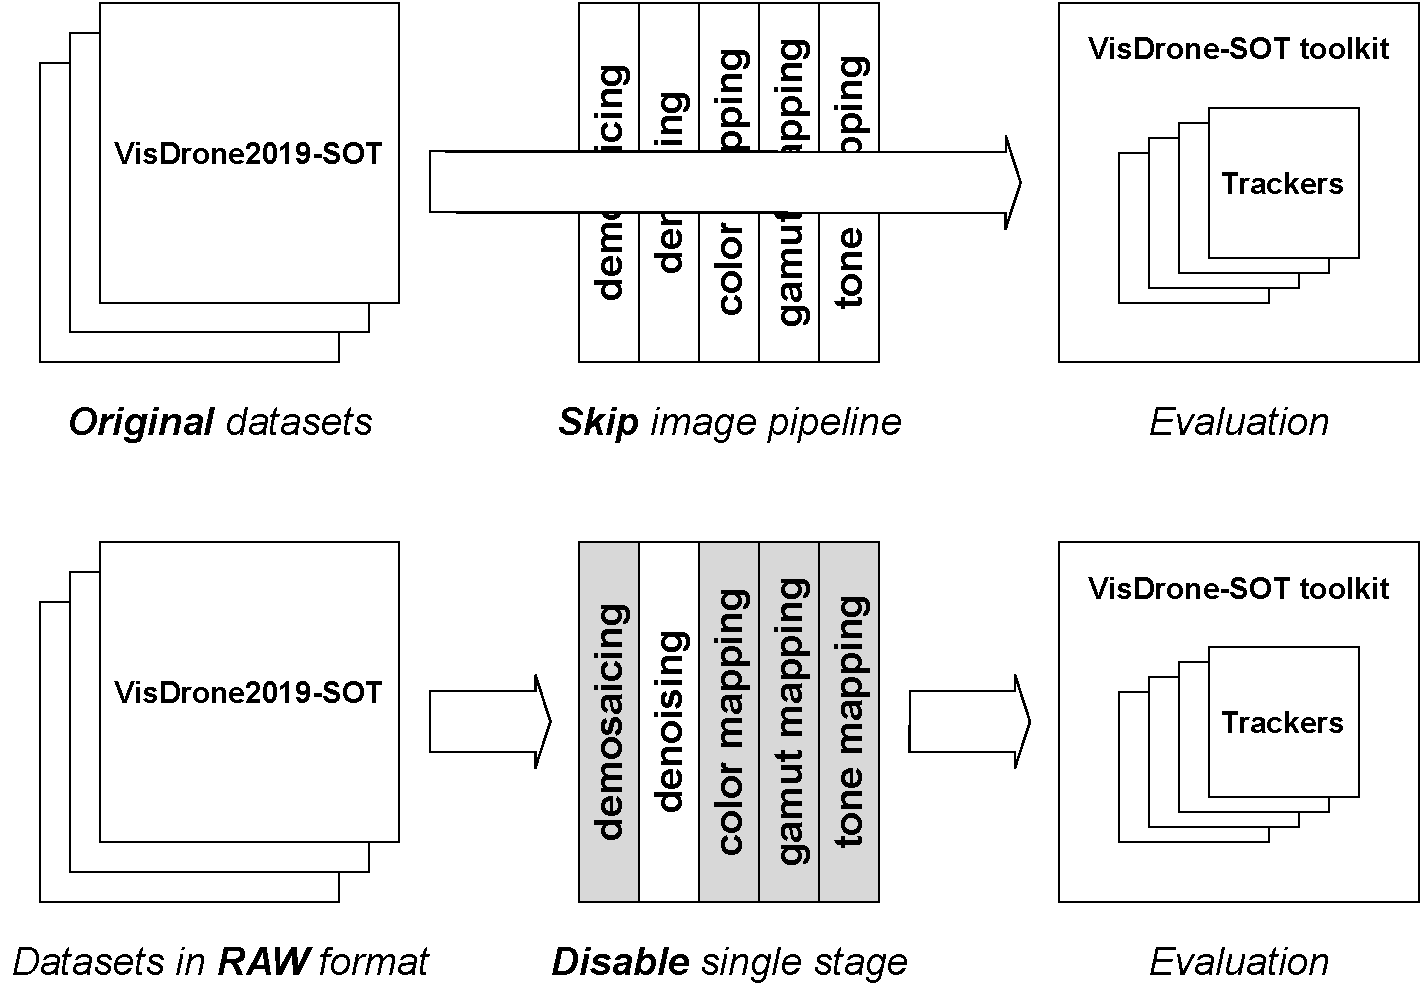
\includegraphics[width=0.8\linewidth]{fig/eva2.pdf}
            \caption{orig. vs. disable single stage}
        \end{center}
    \end{figure}
\end{frame}

\subsection{Evaluation}

% PRE & AUC
\begin{frame}
    \begin{figure}[htpb]
        \begin{center}
            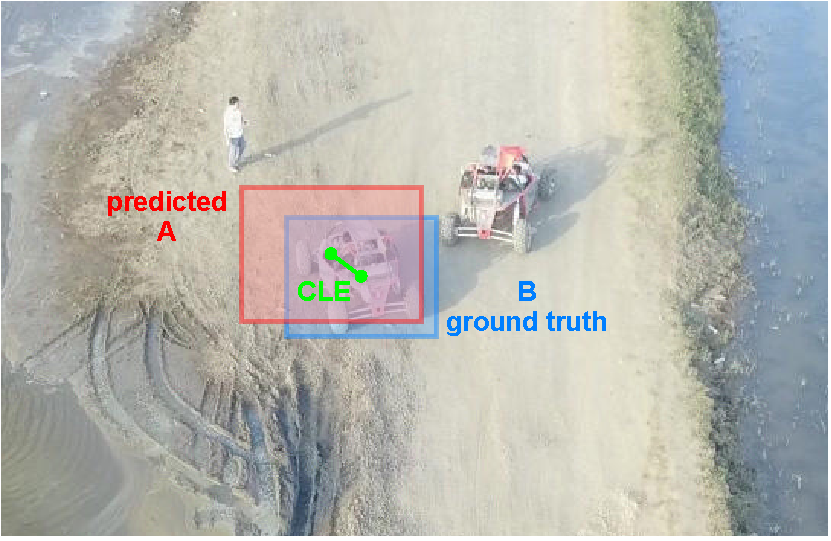
\includegraphics[width=0.8\linewidth]{fig/CLE.pdf}
            \caption{Definition of CLE}
        \end{center}
    \end{figure}
\end{frame}

\begin{frame}
    \begin{figure}[htpb]
        \begin{center}
            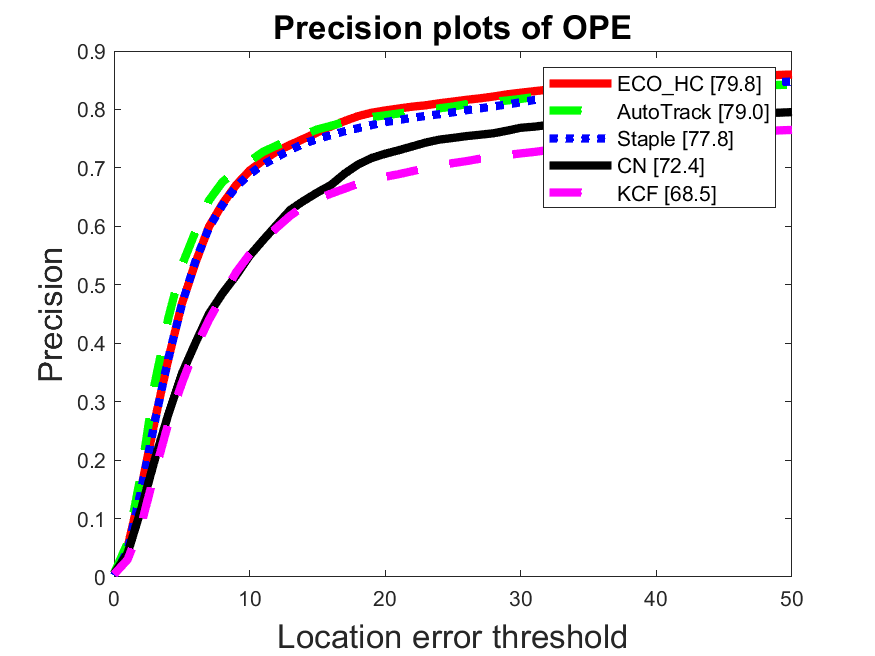
\includegraphics[width=0.8\linewidth]{fig/pre.png}
            \caption{Precision Plot}
        \end{center}
    \end{figure}
\end{frame}

\begin{frame}
    \begin{figure}[htpb]
        \begin{center}
            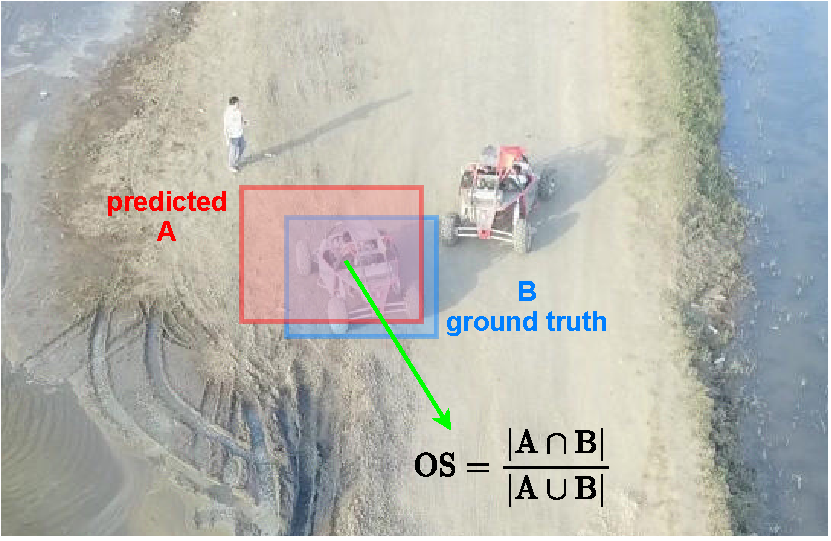
\includegraphics[width=0.8\linewidth]{fig/OS.pdf}
            \caption{Definition of OS}
        \end{center}
    \end{figure}
\end{frame}

\begin{frame}
    \begin{figure}[htpb]
        \begin{center}
            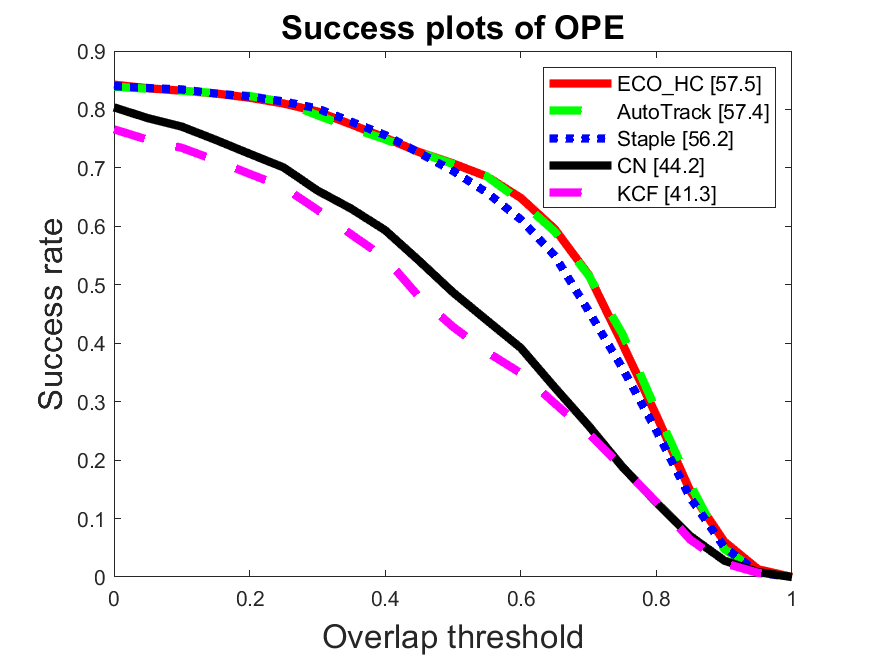
\includegraphics[width=0.8\linewidth]{fig/auc.png}
            \caption{Success Plot}
        \end{center}
    \end{figure}
\end{frame}

% VisDrone-SOT-Toolkit
\begin{frame}
    \begin{itemize}[<+-| alert@+>]
        \item Under one-pass evaluation (OPE)
        \item Using the precision score at threshold = 20
        \item and the area under curve (AUC) of each success plot
    \end{itemize}
\end{frame}

\subsection{Results}

\begin{frame}
    \begin{figure}[htpb]
        \begin{center}
            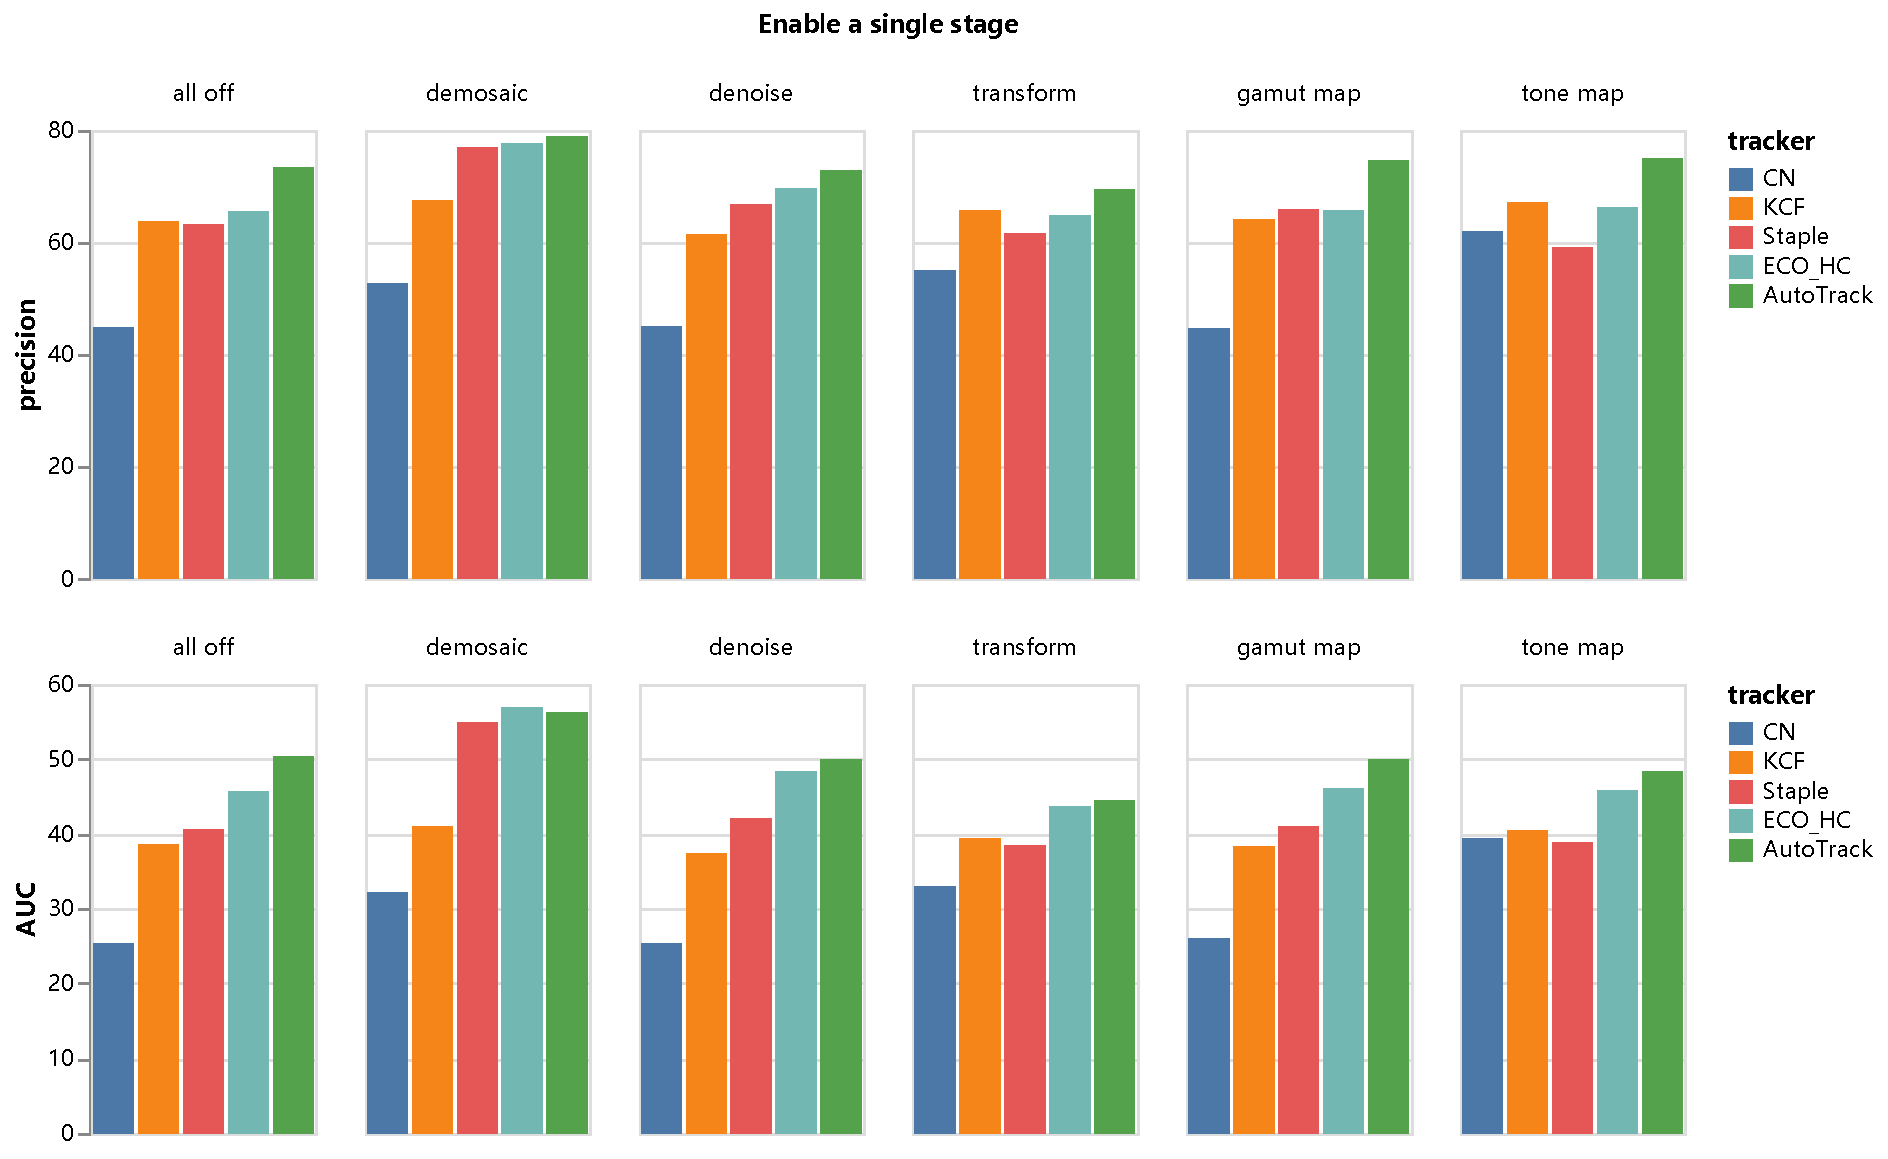
\includegraphics[width=0.8\linewidth]{fig/en.pdf}
            \caption{all off vs. enable single stage}
        \end{center}
    \end{figure}
\end{frame}

\begin{frame}
    \begin{figure}[htpb]
        \begin{center}
            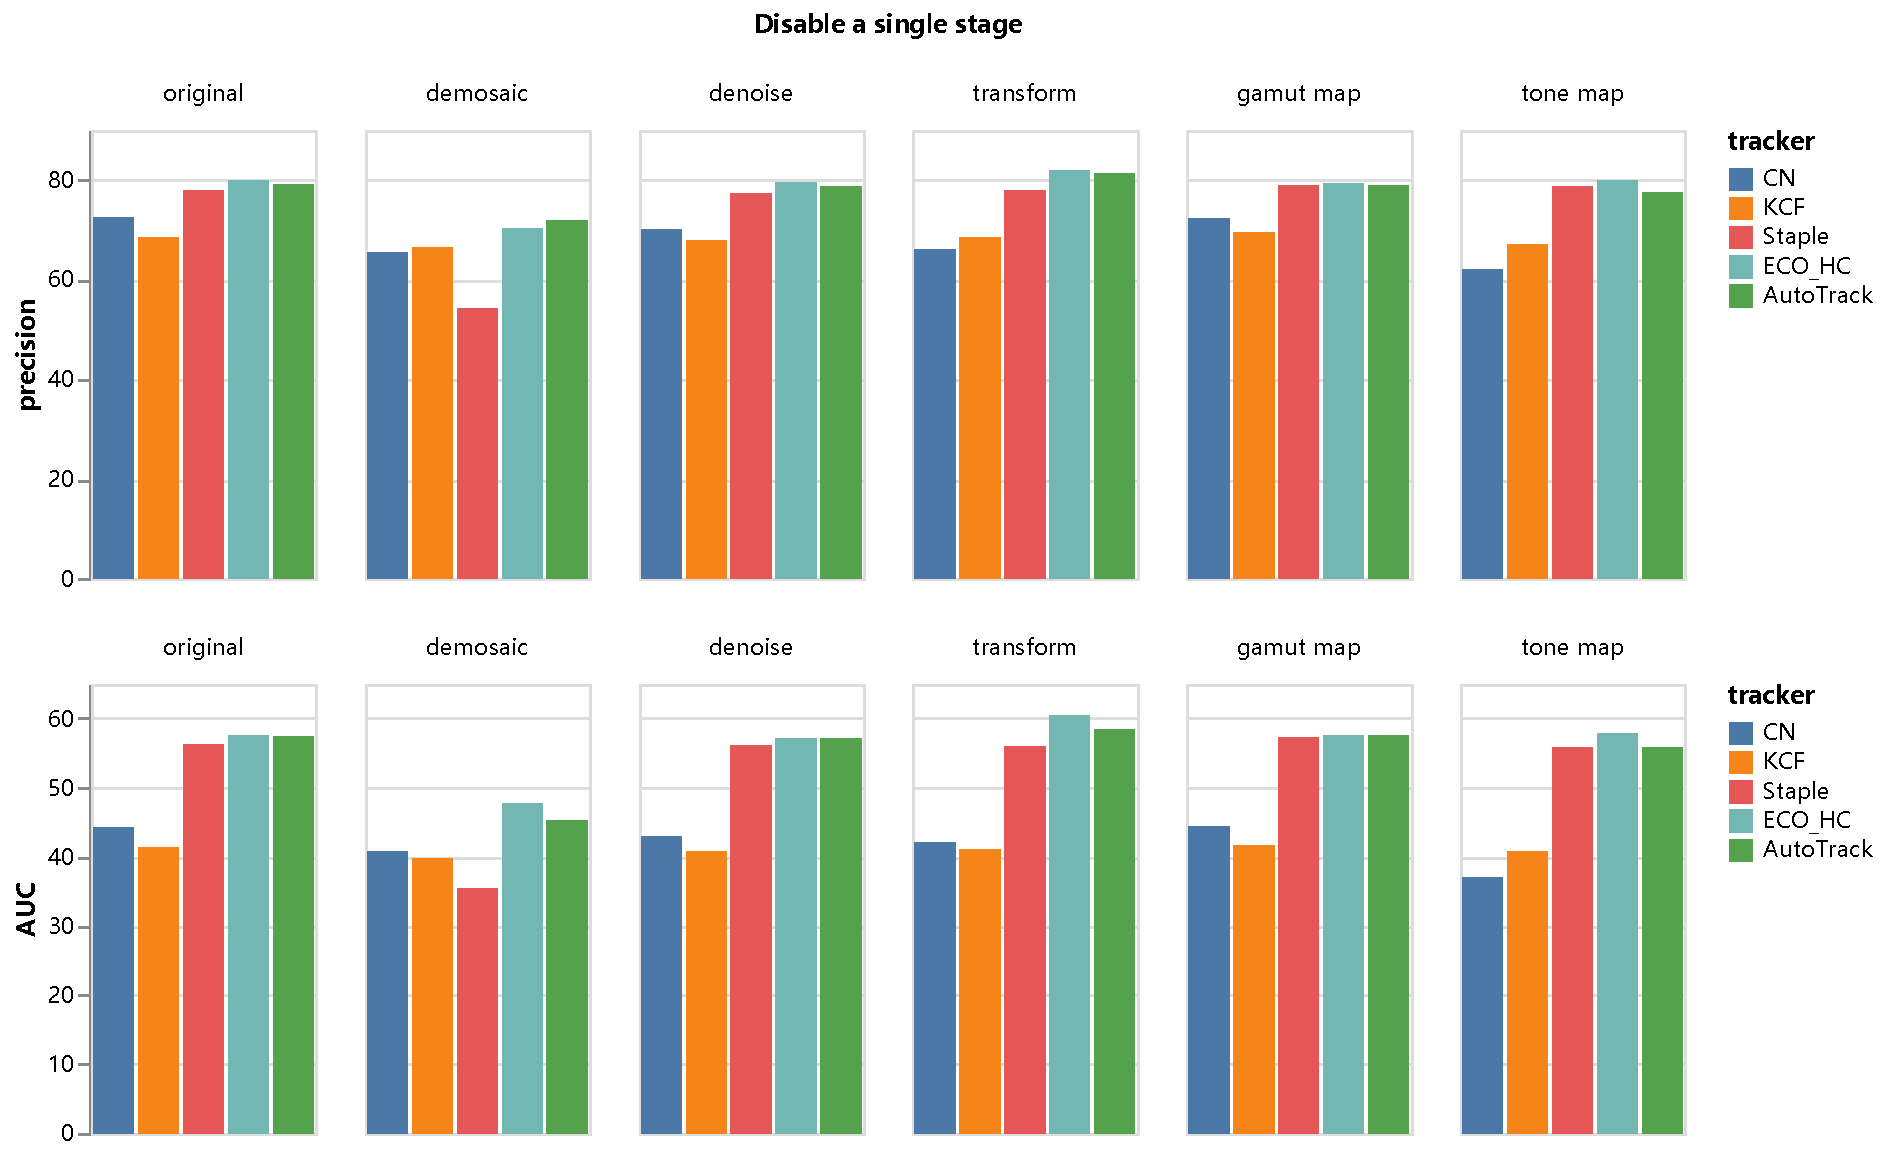
\includegraphics[width=0.8\linewidth]{fig/dis.pdf}
            \caption{orig. vs. disable single stage}
        \end{center}
    \end{figure}
\end{frame}

\begin{frame}
    \begin{figure}[htpb]
        \begin{center}
            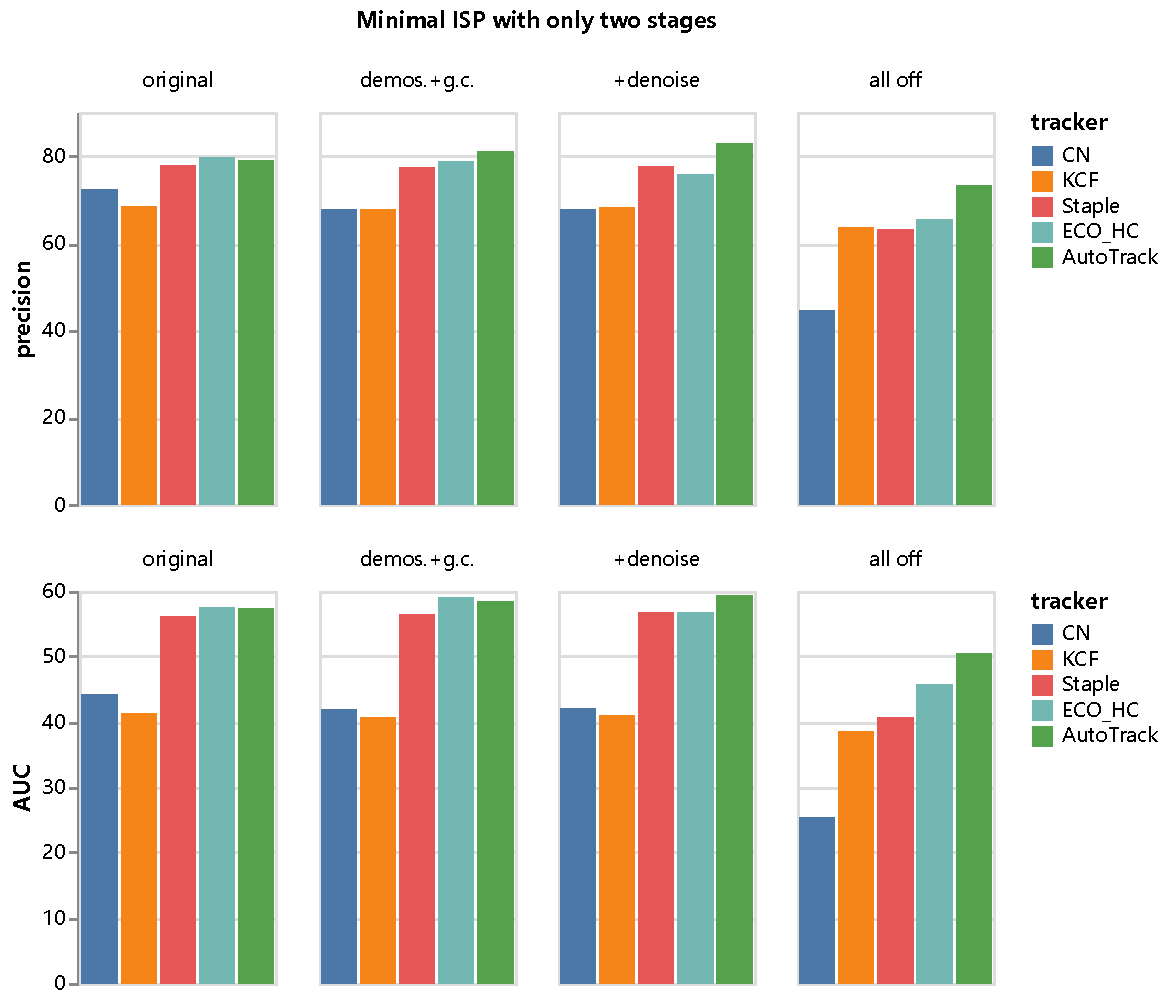
\includegraphics[width=0.7\linewidth]{fig/mini.pdf}
            \caption{Minimal ISP with only two stages}
        \end{center}
    \end{figure}
\end{frame}

\begin{frame}
    \begin{itemize}[<+-| alert@+>]
        \item Only the demosaicing has the greatest impact on the algorithm performance, followed by the gamma transform.
        \item The demosaicing stage will smooth the noise, resulting in a denoising effect\footfullcite{lubana2019minimalistic}.
    \end{itemize}
\end{frame}

\subsection{Ideas of ISP Designing}

\begin{frame}
    \begin{figure}[htpb]
        \begin{center}
            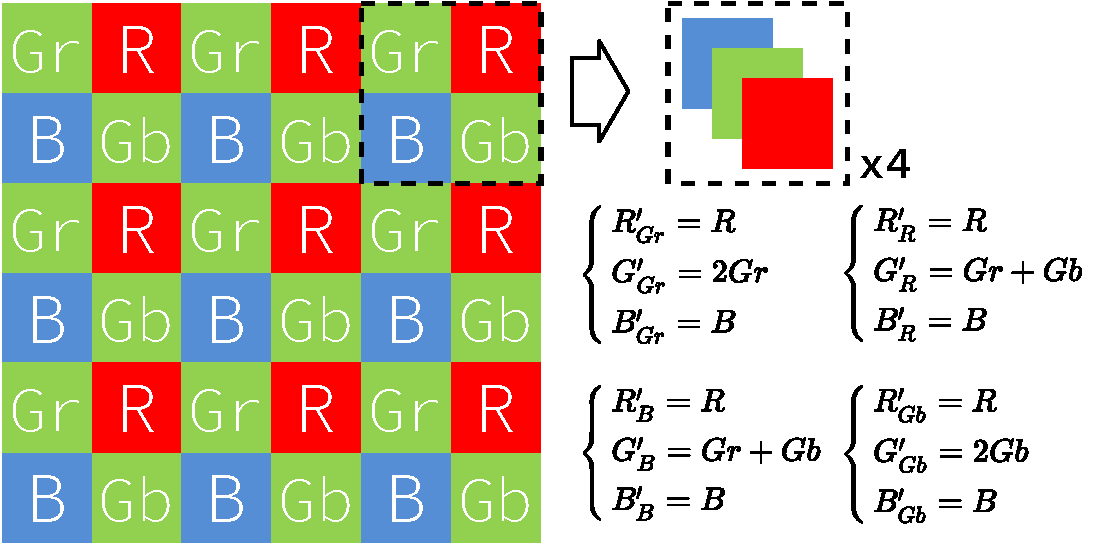
\includegraphics[width=0.8\linewidth]{fig/isp_dem_1.pdf}
            \caption{Use Subsampling to approximate Demosaicing}
        \end{center}
    \end{figure}
\end{frame}

\begin{frame}
    \begin{figure}[htpb]
        \begin{center}
            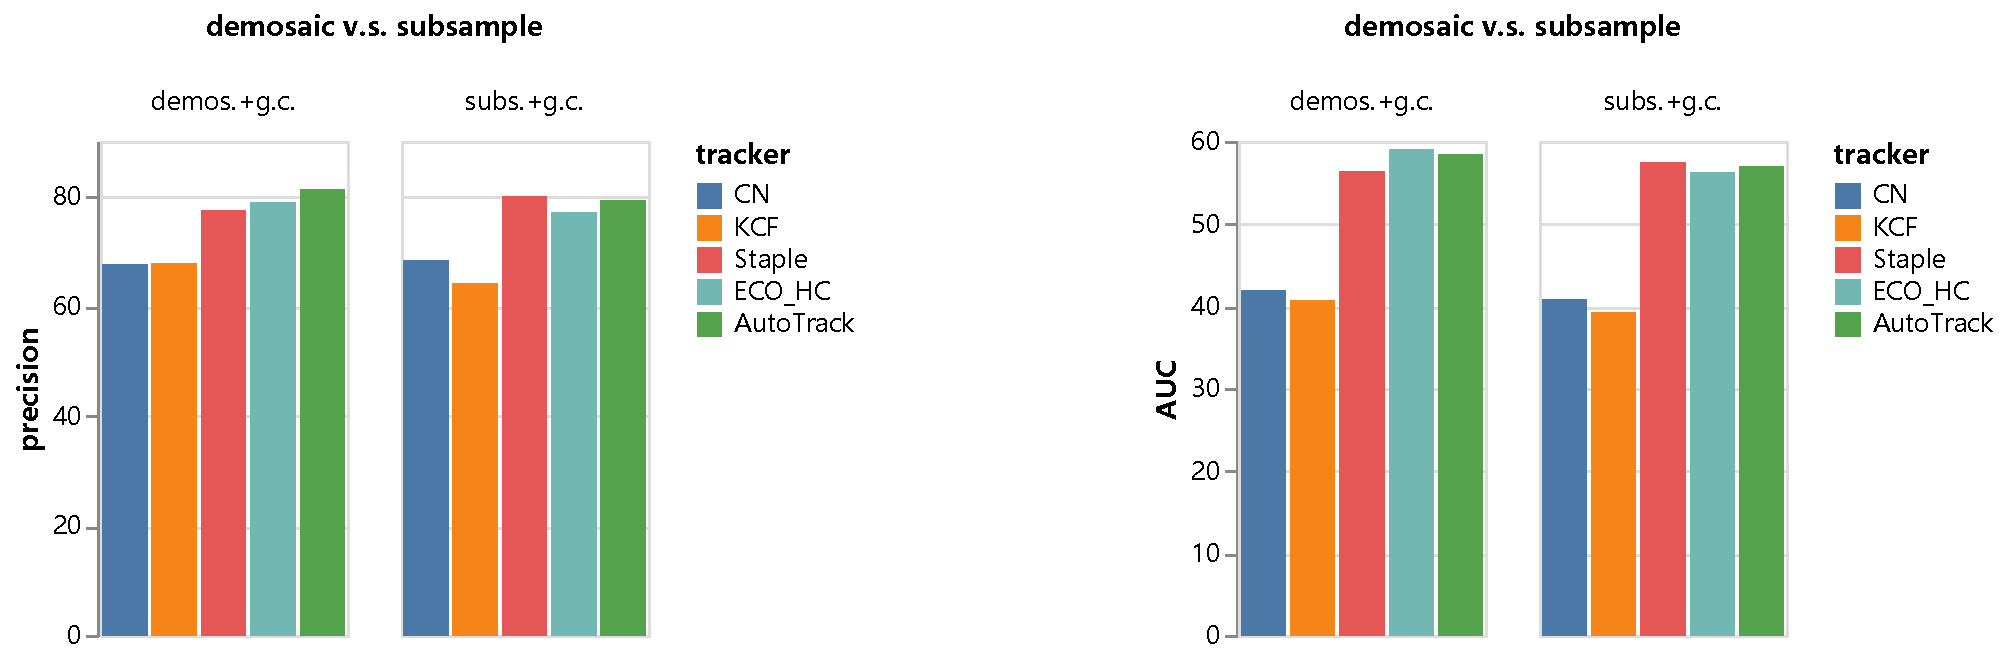
\includegraphics[width=0.8\linewidth]{fig/isp_dem_2.pdf}
            \caption{Demosaicing vs. Subsampling}
        \end{center}
    \end{figure}
\end{frame}

\begin{frame}
    \begin{figure}[htpb]
        \begin{center}
            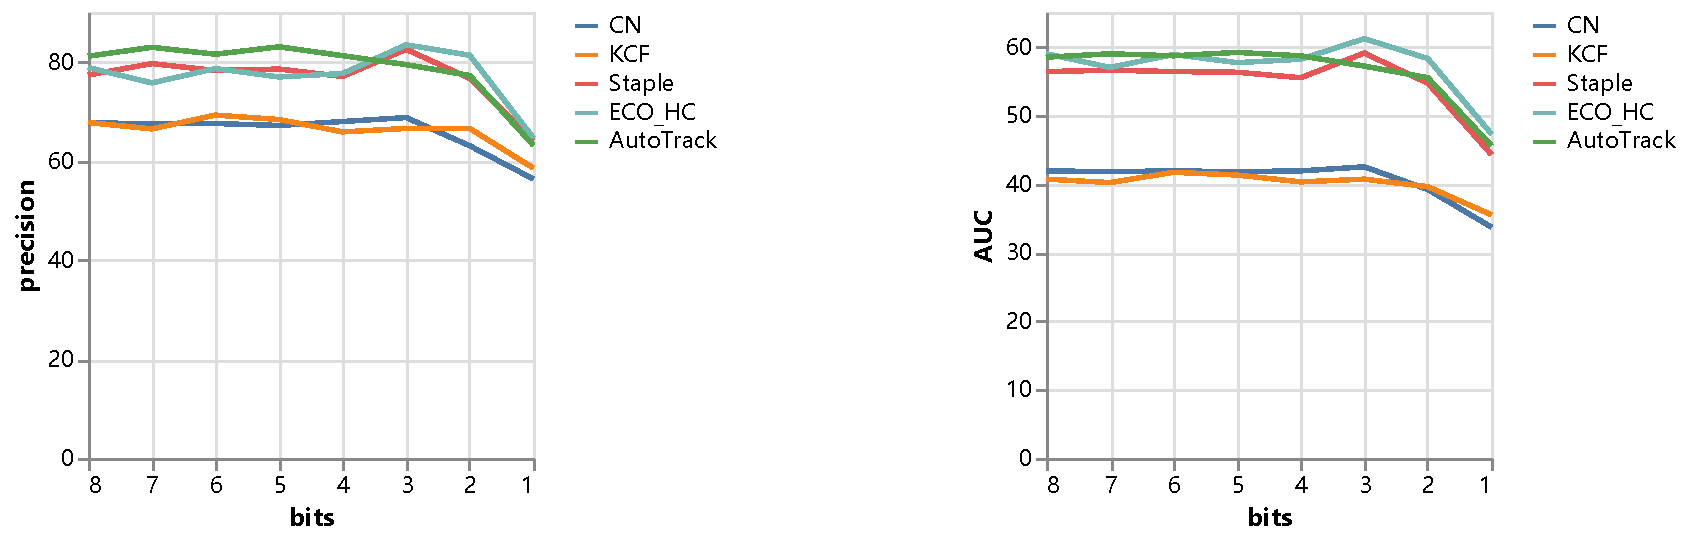
\includegraphics[width=0.8\linewidth]{fig/bits.pdf}
            \caption{Logarithmic quantization}
        \end{center}
    \end{figure}
\end{frame}

\begin{frame}
    \begin{figure}[htpb]
        \begin{center}
            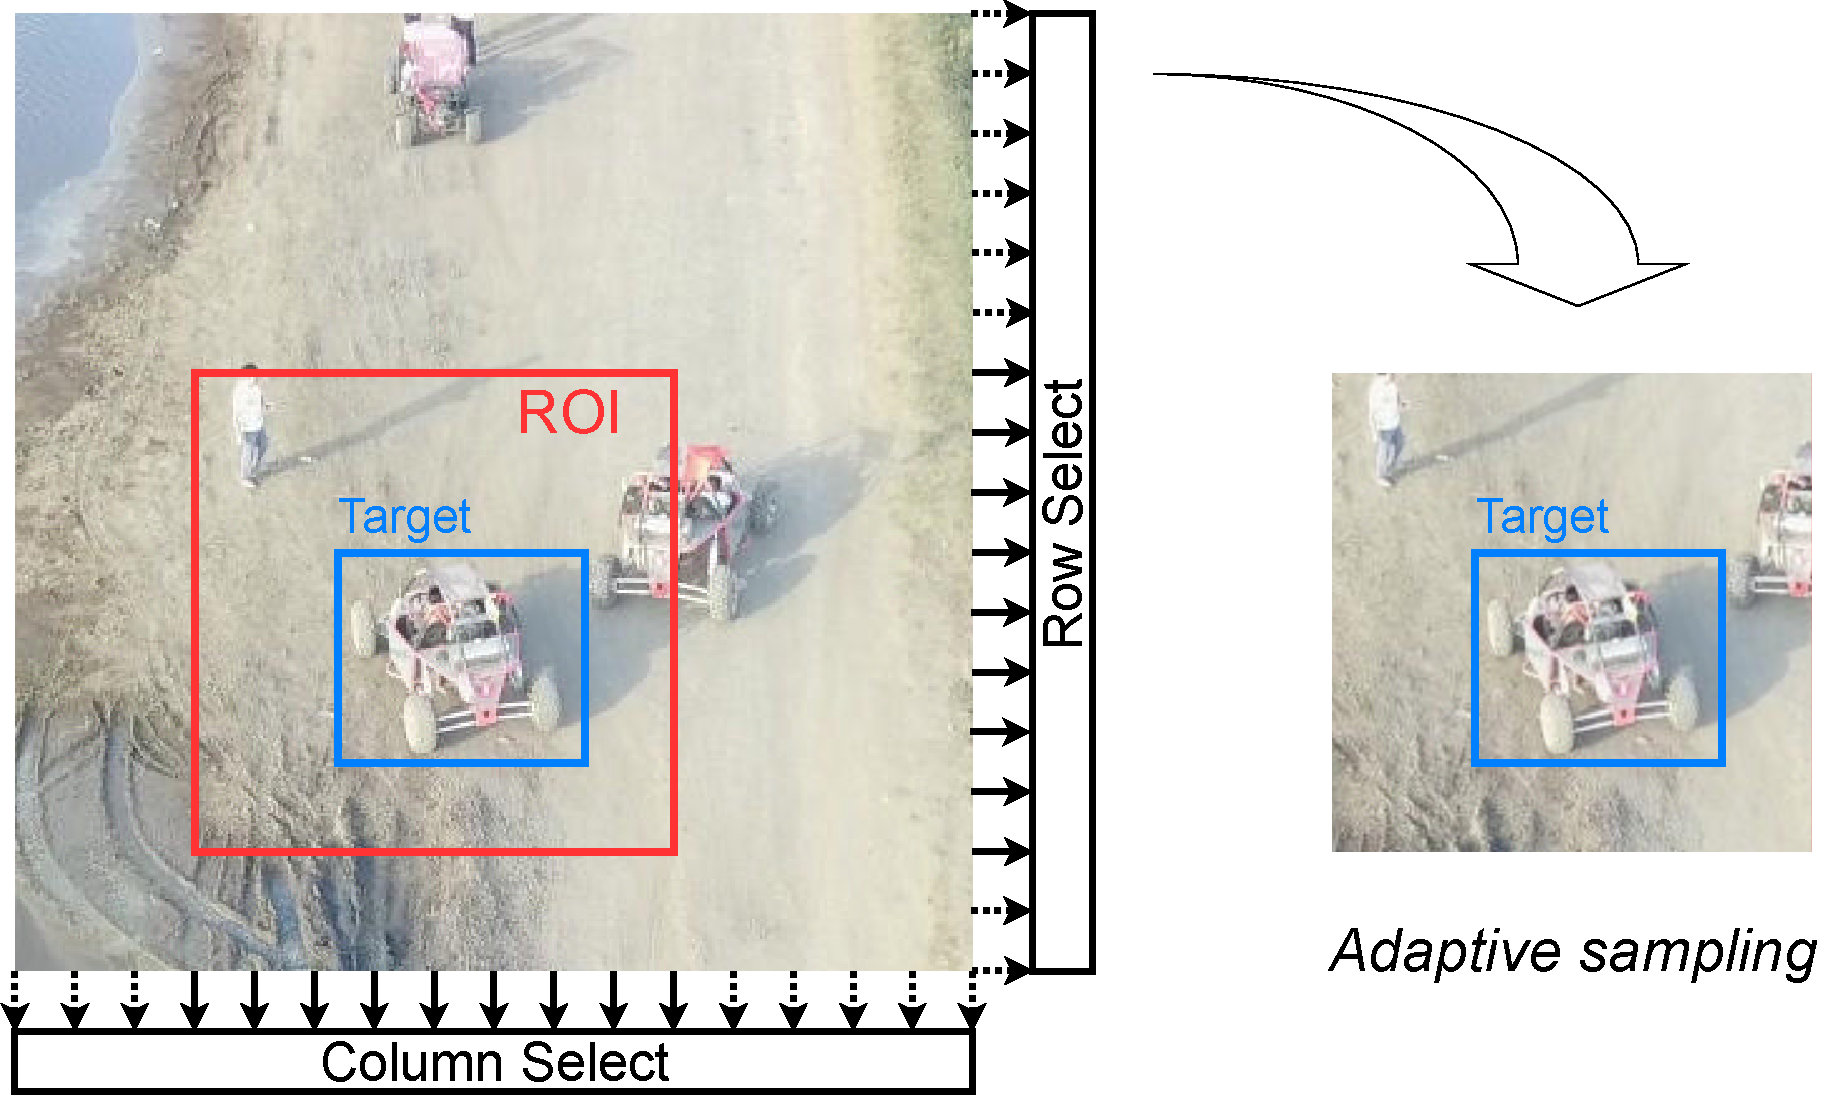
\includegraphics[width=0.7\linewidth]{fig/ad_s.pdf}
            \caption{Adaptive Sampling}
        \end{center}
    \end{figure}
\end{frame}

\section{Highlights}

\begin{frame}
    \begin{itemize}[<+-| alert@+>]
        \item Based on related work, the sensitivity of the performance of a series of DCF-based trackers to different stages of the imaging pipeline in the UAV scenario is tested for the first time.
        \item Based on the above experiment results, the hardware implementation idea of the minimum imaging pipeline is discussed
        \item In addition, an effective optimization scheme is proposed to address the problem of the tedious and time-consuming datasets conversion process in the experiment.
    \end{itemize}
\end{frame}

\section{Discussion}

\begin{frame}
    \begin{itemize}[<+-| alert@+>]
        \item Limitation: only a limited dataset and tracking algorithm were tested, and the proposed ideas of ISP designing are not tested in hardware.
        \item Future Work: We will use more datasets and trackers to verify the above conclusions, and will design corresponding hardware implementations for testing.
    \end{itemize}
\end{frame}

% final frame
\begin{frame}
    \begin{center}
        {\Huge\calligra Thanks!}
    \end{center}
\end{frame}

\end{document}
